\documentclass[12pt, a4paper]{report}
\usepackage[utf8]{inputenc}
% hyperref
\usepackage[bookmarks, colorlinks, breaklinks]{hyperref}  % PDF hyperlinks, with coloured links
\hypersetup{linkcolor=black, citecolor=black, filecolor=black, urlcolor=black} % black links, for printed output
\usepackage{graphicx}

\def\chapterautorefname{Chapter}

\begin{document}
\title{Requirements Analysis and Specification Document: myTaxiService}
\author{Chitti Eleonora, De Nicolao Pietro, Delbono Alex}
\date{\today}
\maketitle
\tableofcontents

%%%%%% INTRODUCTION %%%%%%%%
\chapter{Introduction}
\label{ch:introduction}

\section{Purpose}
\section{Purpose}
\label{sec:purpose}

%TODO Alex


\section{Scope}
The system is a taxi reservation and dispatching system for large cities. Its aim is to simplify the access of passengers to the service and to guarantee a fair management of taxi queues.

The system consists in a back-end server application (\emph{myTaxi Server}), a web application front-end (\emph{myTaxi Web}) and in a mobile application (\emph{myTaxi Mobile}).

The system has 2 types of users: passengers and taxi drivers; it should allow the users to sign up and login with their credentials.
The system has to know the location of both the passengers and the taxi drivers.

The system allows any passenger to request a taxi, informing him o her of the incoming taxi code and the estimated waiting time.

The system knows about the available taxi drivers and, when a request is incoming, informs one of them about the location of the available passenger; the taxi driver can either accept or deny the ride.
If the taxi driver accepts the ride, the system sends a confirmation to the passenger, together with the estimated waiting time.
If the taxi driver rejects the ride, the system looks for another taxi driver in the same area of the city.

The system offers programmatic interfaces (APIs) to enable the development of additional services on top of the basic one.

The system is provided with two optional modules:
\begin{description}
\item[Taxi reservation] allows the passenger to reserve a taxi by specifying the origin and the destination of the ride.
\item[Taxi sharing] allows the passengers to share a ride together, dividing the costs.
\end{description}


\section{Definitions, acronyms, and abbreviations}
\section{List of Definitions and Abbreviations}
\label{sec:definitions}

\begin{description}
\item[RASD:] Requirements Analysis and Specification Document.
\item[DD:] Design Document.
\item[ITPD:] Integration Test Plan Document (this document).
\item[RDBMS:] Relational Data Base Management System.
\item[DB:] the database layer, handled by a RDBMS.
\item[Application server, business tier or back-end:] the layer which provides the application logic and interacts with the DB and with the front-ends.
\item[Front-end:] the components which use the application server services, namely the web front-end and the mobile applications.
\item[Web server:] the component that implements the web-based front-end. It interacts with the application server and with the users' browsers.
\item[JSF:] JavaServer Faces.
\end{description}


\section{References}
\begin{itemize}
\item Project rules: ``AA 2015-2016 Software Engineering 2 - Project goal, schedule and rules"
\item Assignment: ``Software Engineering 2 Project, AA 2015/2016 - Assignments 1 and 2"
\item IEEE Std 830-1998: ``IEEE Recommended Practice for Software Requirements Specifications"
\end{itemize}

\section{Overview}
\section{Overview}
\label{sec:overview}

This chapter provides a comprehensive view over the system components, both at a physical and at a logical level.

The system will be described starting with high-level components (\autoref{sec:high-level}). This high-level design will be thoroughly dissected and detailed in \autoref{sec:component-view}.
Section~\ref{sec:deployment-view} will put some attention on the deployment of the system on physical tiers, and \autoref{sec:runtime-view} will describe the dynamic behaviour of the software.
Section~\ref{sec:component-interfaces} will focus on the interface between different components of the system.

The design choices and patterns used in the aforementioned sections will be presented and discussed in~\autoref{sec:styles-patterns}.


%%%%%% OVERALL DESCRIPTION %%%%%%%%
\chapter{Overall description}
\label{ch:overall-desc}

\section{Product perspective}
The back-end stores its data in a RDBMS and  can run on every platform that supports the JVM.
The web application works on any web server that supports Java. The mobile application is supported by Android, iOS. The system provides APIs to extend its functionalities, e.g. :
\begin{itemize}
\item taxi reservation
\item ride sharing
\item online payments
\item \ldots
\end{itemize}

%TODO block diagram

%  Alex
\subsection{User interfaces}
The user interfaces must provide the following logical characteristics both in the mobile app and in the web application:
\begin{itemize}
\item The possibility to choose the language used in every moment during every operation.
\item A first screen that lets the user login in order to begin operations.
\item A dashboard with links to every function in order to show the user the capabilities of the system and allow him to save time.
\item A link to the dashboard in every screen.
\item A reminder in the top bar to show the last taxi service called, with a link to a screen which displays the reserved taxi history.
\end{itemize}

\subsection{Hardware interfaces}
The system has to deal with the dichotomy of the web user interaction and the mobile one. It is necessary to provide a common look and feel, without losing simplicity with the different hardware interfaces. For instance, the compilation of data fields has to be made with multiple choices in order to simplify the user's experience of the app. Same goes for the dimension of buttons that can not be too small.

\subsection{Software interfaces}
The required software products used by the systems are:
\begin{itemize}
\item MySQL 5.7   \url{http://dev.mysql.com}
\item Java SE 8   \url{http://java.com}
\end{itemize}
% TODO review Software interfaces and user interfaces for avoiding inconsistency


\section{Product functions}
\begin{figure}
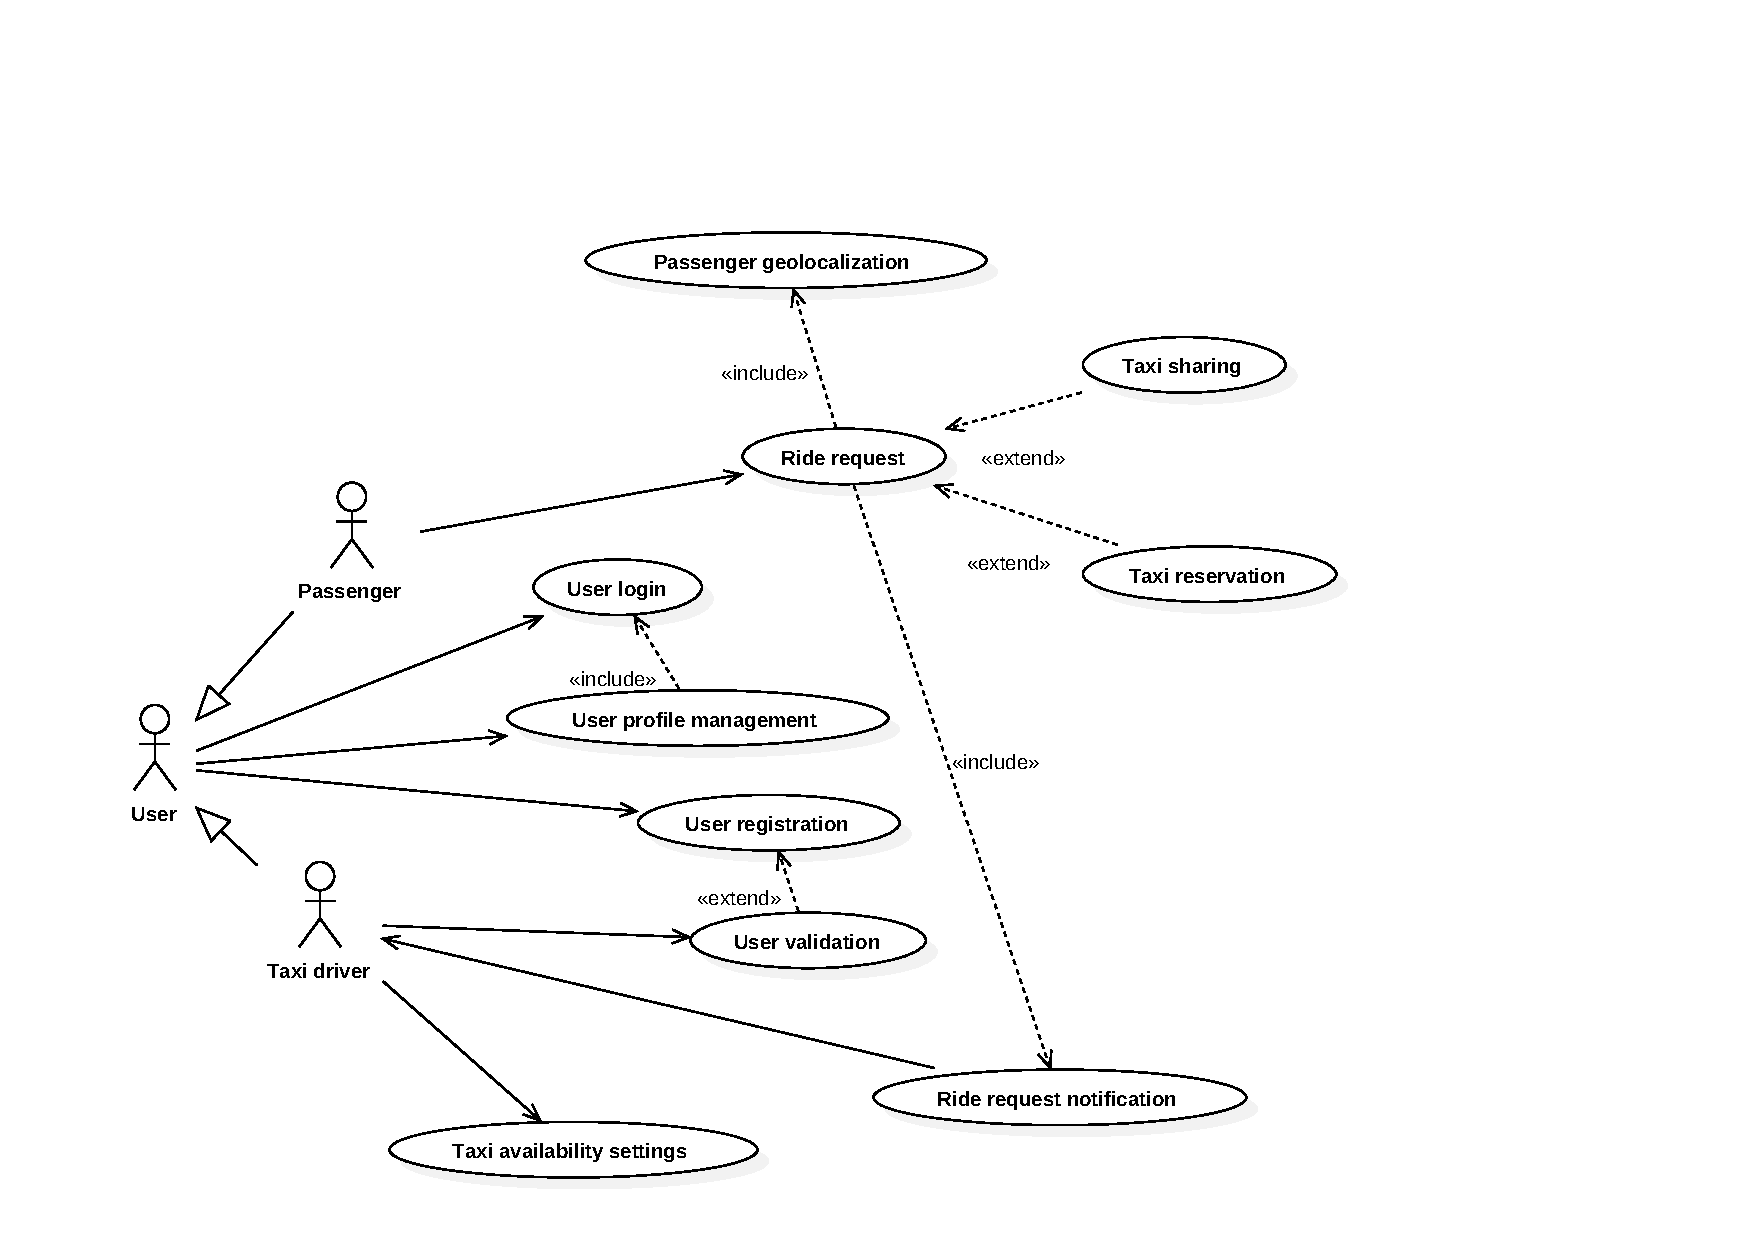
\includegraphics[width=\textwidth]{diagrams/usecase_whole.pdf}
\caption{The comprehensive use-case diagram of all the functionalities implemented by the system.}
\end{figure}

\begin{figure}
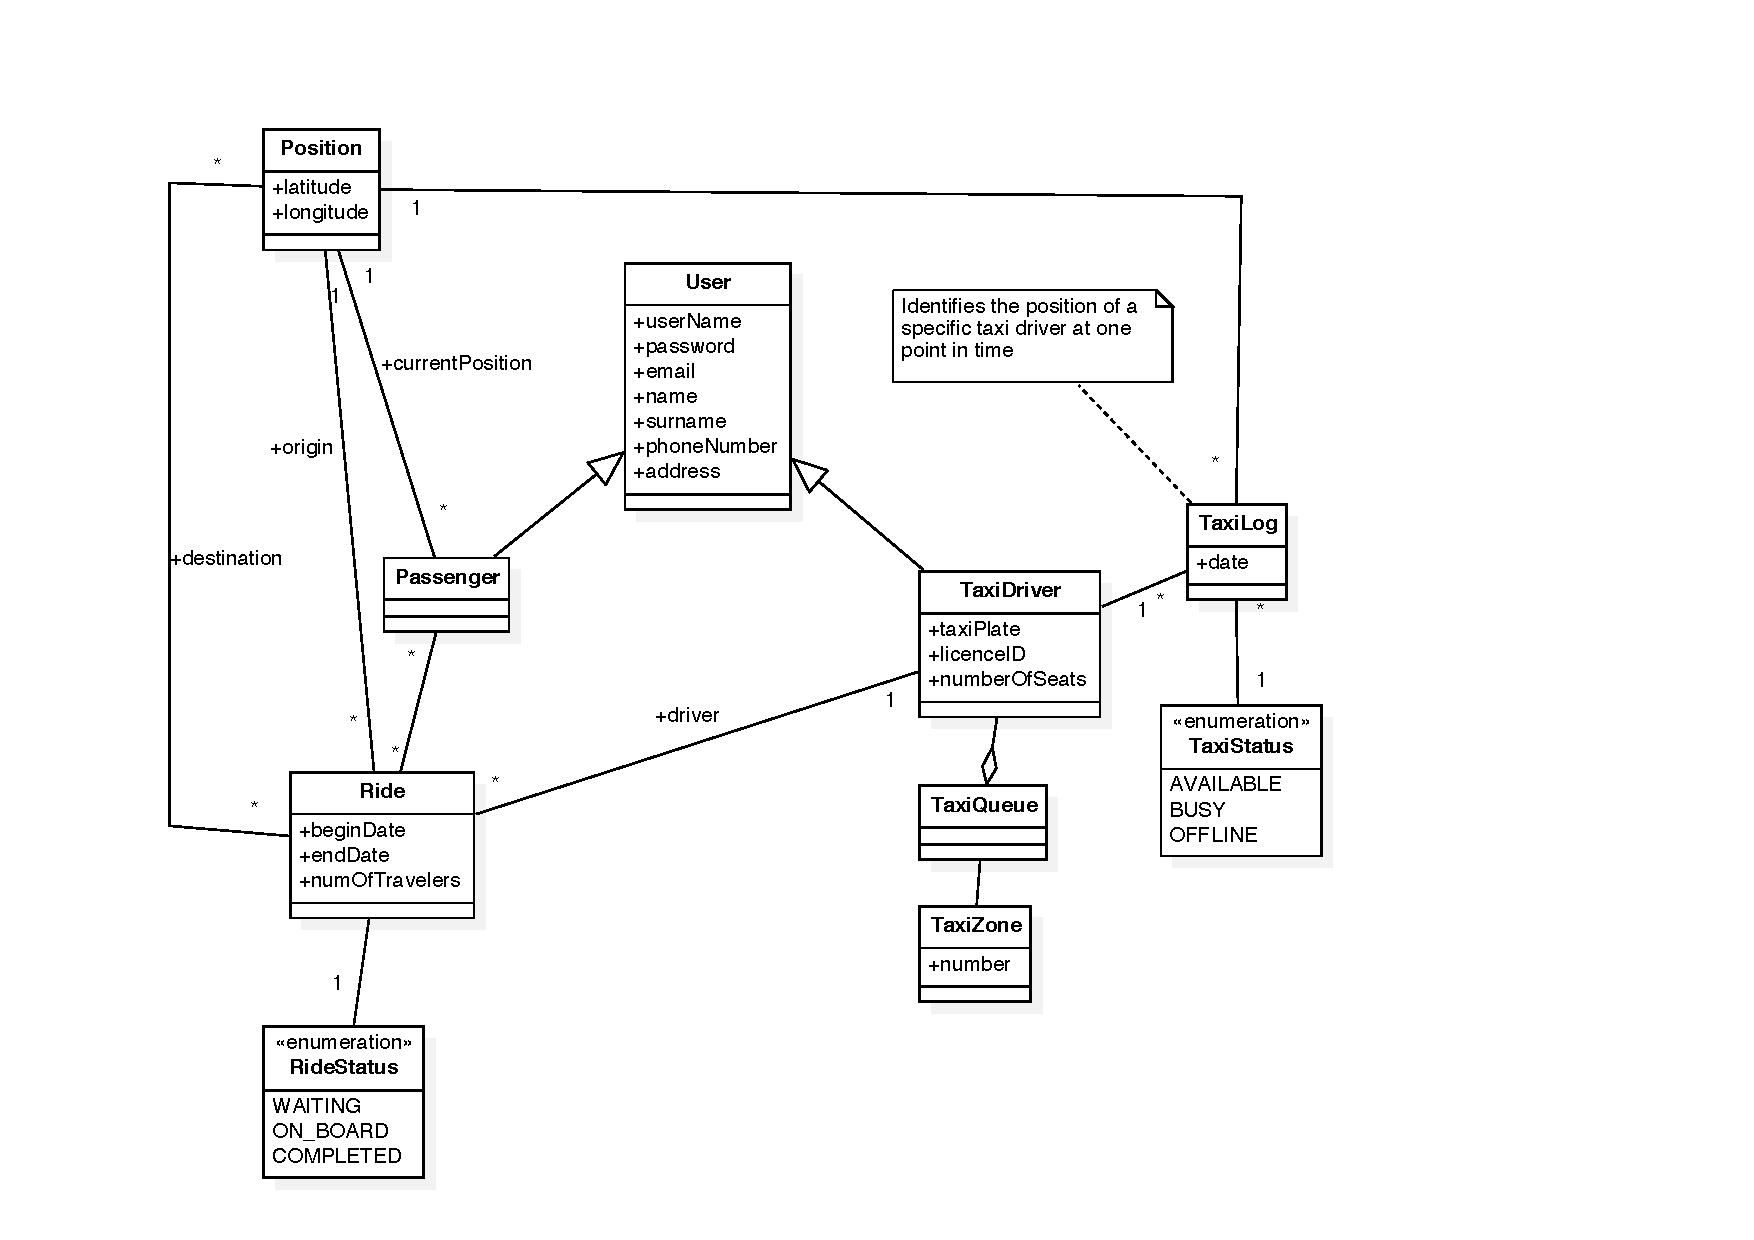
\includegraphics[width=\textwidth]{diagrams/general_class_diagram.pdf}
\caption{The comprehensive class diagram of the system.}
\end{figure}
The system allows passengers to book a taxi, and taxi drivers to take care of the request.

This is a list of what the users of the service can do.
\begin{itemize}
    \item All users can:
        \begin{itemize}
            \item create an account
            \item login
            \item edit profile data
        \end{itemize}
    \item Passengers can:
        \begin{itemize}
            \item request a taxi
            \item share a taxi with other passengers
            \item reserve a taxi in advance for a specific time
        \end{itemize}
    \item Taxi drivers can:
        \begin{itemize}
            \item mark themselves as available or busy
            \item accept or deny a lift request
            \item get the exact position of the passenger, after having accepted a ride request
        \end{itemize}
\end{itemize}


\section{User characteristics}
The two kinds of users are \emph{passengers} and \emph{taxi drivers}.
We give for granted that both kinds of users have access to Internet.

Taxi drivers must be able to install and use the mobile application on their cellphone to answer the ride requests.

Passengers have to use the browser application or the mobile app. They move alone or with other people (``travelers'').


\section{Constraints}
\subsection{Regulatory policies}
It's user responsibility to ensure that the use of the system complies with the local laws and policies.

The system must ask the user for the permission to acquire, store and process personal data and web cookies. The system must offer to the user the possibility to delete all the personal data.

\subsection{Hardware limitations}
the system has to run under the following conditions:
\begin{itemize}
\item App
\begin{itemize}
\item 3G connection, at 2 Mb/s
\item 100 MB of free space
\item 2 GB of RAM
\end{itemize}
\item Web application
\begin{itemize}
\item 2 Mb/s Internet connections
\item 800x600 resolution
\end{itemize}
\end{itemize}

\subsection{Reliability requirements}
The system must have a minimum availability of 98\%.

\subsection{Criticality of the application}
The system is not employed in life-critical applications.

\subsection{Safety and security considerations}
The locations of the passenger and its destinations must be kept private unless the passenger chooses to share rides.

Only taxi drivers with a valid license must be able to use the service for security reasons.


\section{Assumptions and dependencies}
We assume that:
\begin{itemize}
\item the taxi driver's cellphone is provided with a GPS navigator;
\item the GPS on the mobile phone of the taxi driver is available.
\item the taxi has to be in the taxi zone queue.
\item The GPS position of the taxi driver must be in the same area of the user's.
\item the taxi driver is able to reach the meeting point within 10 minutes from the given hour 90\% of the times;
\item the taxi driver is able to reach the meeting point within 20 minutes from the given hour 100\% of the times;
\item the passenger waits in the location until the taxi arrives;
\item the taxi driver picks up the correct passenger;
\item the taxi driver correctly updates his status (off shift, available, busy);
\item the passenger specifies the correct location.
\item the taxi driver is able to see notifications of new passengers during sharing rides.
\item the passenger specifies the correct destination when ride sharing is enabled
\item the user is willing to modify his route, though not greatly, in order to allow ride sharing.
\end{itemize}


\section{Future extensions}
% alex
The system will be implemented in order to offer the possibility of further extensions, for example:

\begin{enumerate}
    \item Provide secure and reliable methods for ride payments. This functionality allow the passengers to pay for the rides using credit card information stored in a secure way in their profiles.
    \item Offer a taxi rating system which lets the passengers evaluate taxi drivers.
    \item Monitor passengers' reliability, recording when they do not show up at the meeting point or how many minutes later they arrive, in order to limit their access to the service when their reliability is bad.
    \item Create a fidelity score for every passenger, which gives them the opportunity to benefit from special offers. The score increases every time the passenger uses of the taxi service, proportionally with the distance covered.
\end{enumerate}


%%%%%% SPECIFIC REQUIREMENTS %%%%%%%%
\chapter{Specific requirements}
\label{ch:requirements}

\section{External interface requirements}
\subsection{User interfaces}

The user interfaces must satisfy the following UI constraints:
\begin{itemize}
    \item Web application
        \begin{enumerate}
        \item The web pages must adhere to the W3C standards. In particular, the software shall conform to the HTML~5~\cite{w3c-html5} and CSS~\cite{w3c-css} standards.
        \item The web pages must be accessible also by text-only browsers.
        \end{enumerate}
    \item Mobile app
        \begin{enumerate}
        	\item The iOS version must adhere to the iOS Human Interface Guidelines~\cite{apple-ios-hig}.
	\item The Android version must follow Android design guidelines~\cite{google-android-hig}.
        \end{enumerate}
     \item Server back-end
     	\begin{enumerate}
		\item The server back-end must be configurable by means of a configuration text file.
	\end{enumerate}
    \item Common to all client interfaces:
    \begin{enumerate}
        \item The clients must have an UI that is accessible to disabled people.
        \item The interface must offer the possibility to choose the language used at all times.
        \item The first screen must ask the user to login in order to begin operations.
        \item A dashboard with links to every function shall be displayed in the home page in order to show the user the capabilities of the system and allow him to save time.
        \item The dashboard must be linked in every screen.
        \item The top bar must show the last taxi service called, with a link to a screen which displays the reserved taxi history.
        \item The compilation of data fields has to be made with suitable controls (multiple choice, date picker, text field, \ldots) in order to simplify the user's experience of the app.
        \item UI controls and views must be suitable for the input interface and the screen size.
    \end{enumerate}
\end{itemize}

\subsection{Hardware interfaces}

The client app must be able to access the GPS data of the user's phone.
It has to deal with security dialogs, authorization and platform-specific standards.

\subsection{Software interfaces}
The system is built in a modular fashion: the core part of the system exposes public APIs allowing the building of new interfaces and modules.

For a detailed specification of the programmatic interfaces, see \autoref{sec:api}.

The required software products used by the back-end are:
\begin{itemize}
\item MySQL 5.7\footnote{\url{http://dev.mysql.com}}
\item Java SE 8\footnote{\url{http://java.com}}
\end{itemize}

\subsection{Communications interfaces}
The clients communicate with the server via HTTPS requests (port 443).


\section{System features}
\subsection{User registration}
\label{user-registration}
\subsubsection{Purpose}
Any user can subscribe through the web application or the mobile app.

In both cases the user has to fill a registration form and must agree to the personal data policy according to his/her country privacy laws, otherwise the registration request shall be aborted.

As soon as the user has submitted all the data, the system verifies the consistency of the information and a confirmation mail is sent to check the availability of the email-address.  After this last check the registration ends successfully.

The system has two kind of registration forms (for the two kinds of registered users): one for passengers and one for taxi drivers.

The taxi driver registration is more restrictive and requires more user information.
The system registers a user that claims to be a taxi driver only if he/she is able to prove it with a currently valid taxi license.


\subsubsection{Scenario 1}
Alice, a normal citizen without a car, has just discovered the existence of myTaxiService web application and she wants to use it.
She opens the homepage of myTaxiService on the website and clicks on ``passenger registration''.

She gives all the information required and authorises the personal data treatment.

The system verifies the submitted information and sends a confirmation mail.
Alice checks the mailbox, opens the mail and clicks on the ``confirm e-mail'' link.

The system informs Alice that the registration succeeded.

\subsubsection{Scenario 2}
Bob is a taxi driver that wants to subscribe to myTaxiService application.
He downloads the mobile application from his phone app-store and once he opens it, he selects ``taxi driver registration''.
He fills the form, enters his license ID and authorises the personal data treatment.

However he forgets to write his phone number on the form so the system warns him about the forgetfulness.
Only after the complete and correct filling of the form, and the personal data treatment authorisation, the registration is one step near the successfully end.

The system verifies the information submitted and sends a confirmation mail.
Bob checks the mailbox, opens the mail and clicks on ``confirm e-mail''.

The system informs Bob that the registration has ended successfully.

\begin{figure}
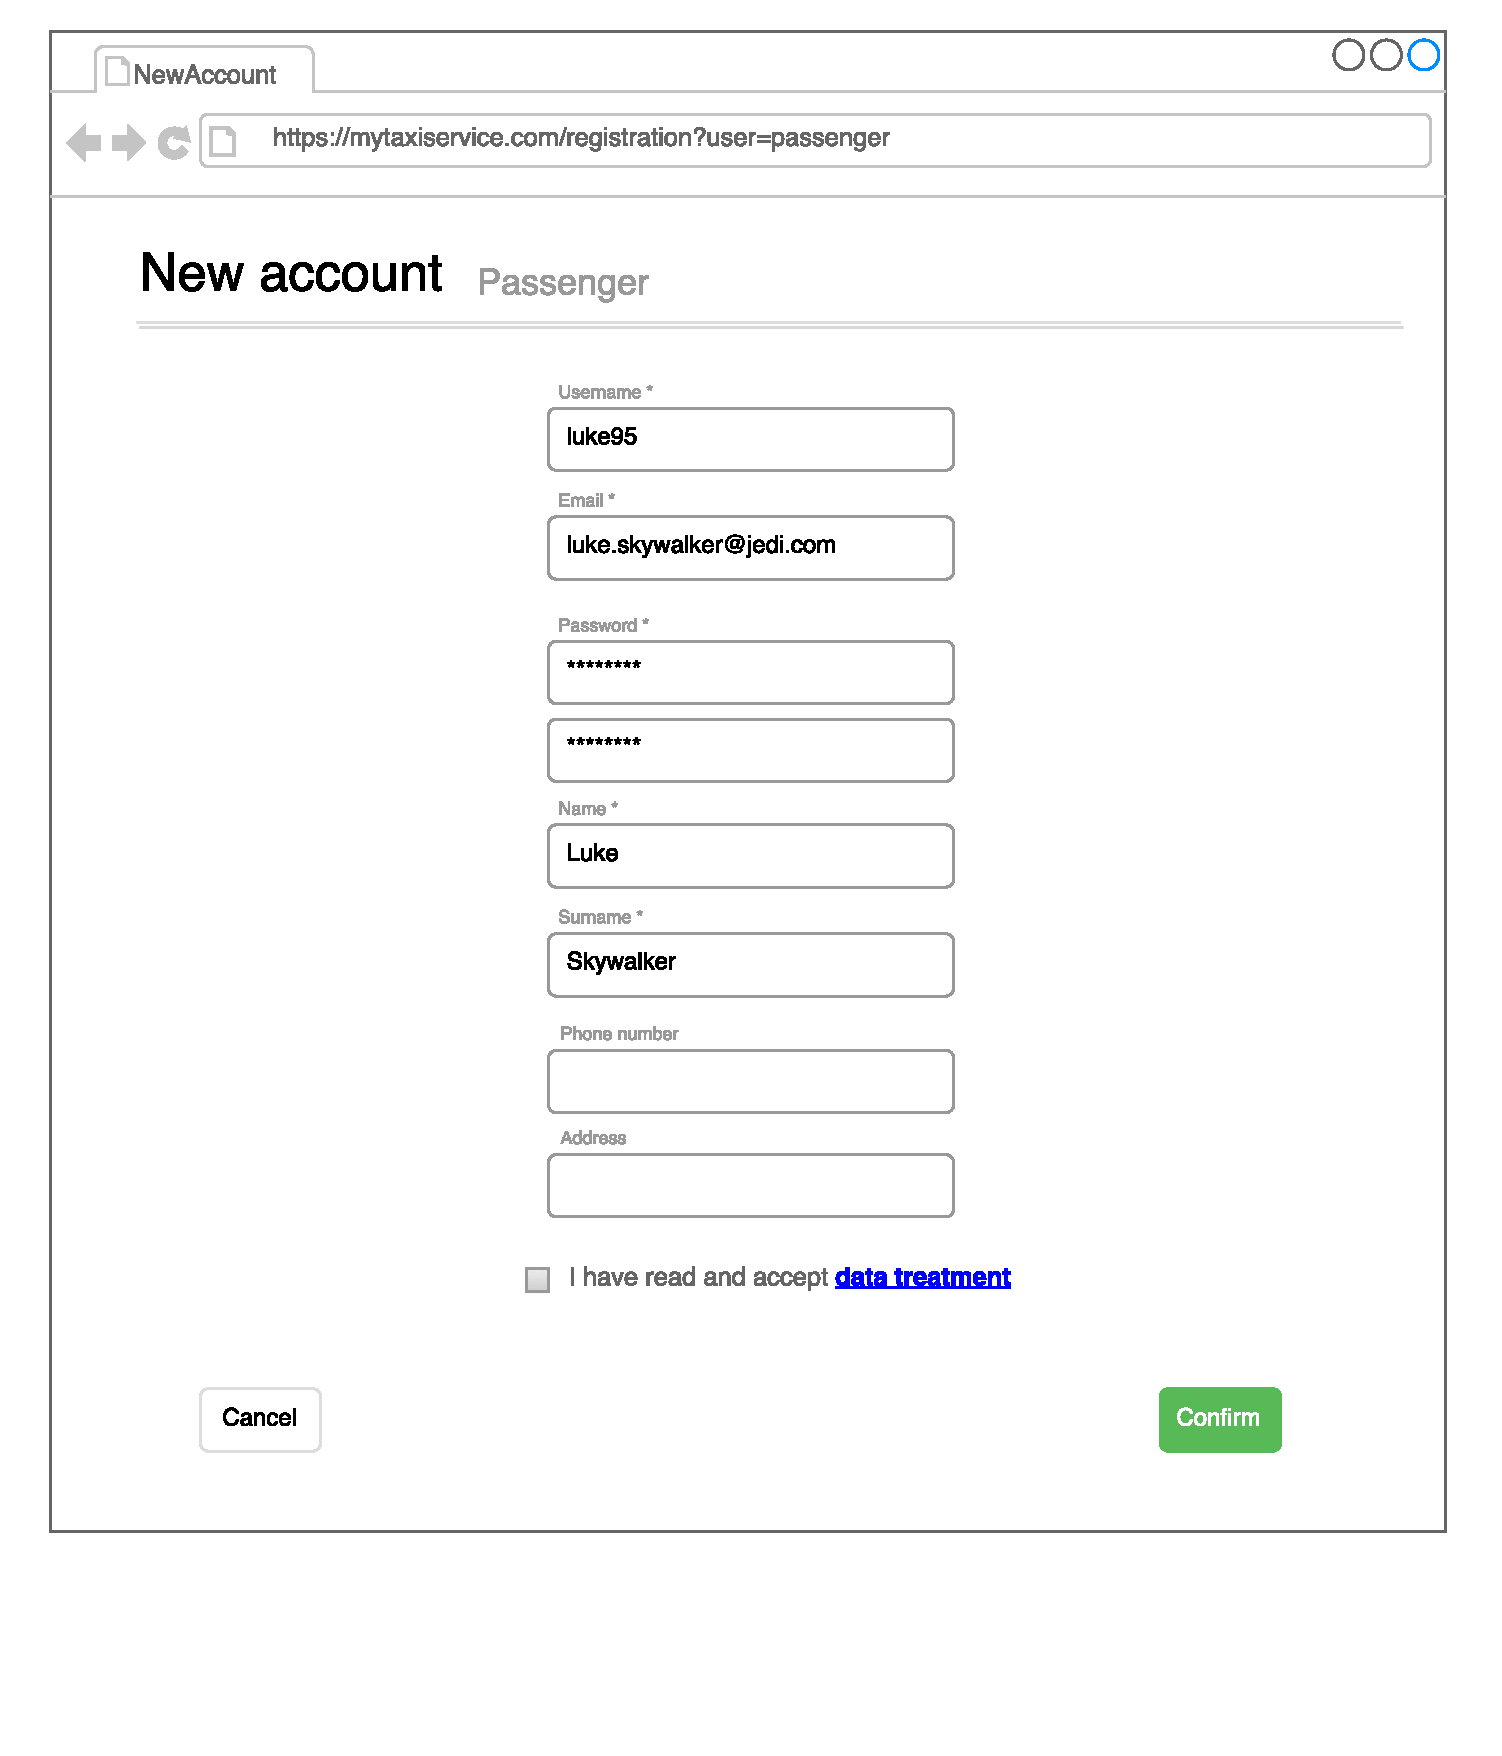
\includegraphics[width=\textwidth]{mockup/Registration.pdf}
\caption{Concept of the registration webpage.}
\label{fig:mockup-registration}
\end{figure}


\subsubsection{Use case}
The use case for user registration is shown in~\autoref{usecase-registration}.

\begin{table}
\begin{center}
\begin{tabular}{| l | p{0.6\textwidth} |}
\hline
Actor & Unregistered user, Registered passenger or taxi driver \\
\hline
Goal & Goal ~\ref{g-login}
\\
\hline
Input condition & The user chooses to create a new user account.  \\
\hline
Event Flow & \begin{enumerate}
	\item The user selects taxi driver or passenger registration.
	\item The registration form is loaded and the user compiles it.\label{load-registration}
	\item The user authorizes the personal data treatment.
	\item The user reads the e-mail received by myTaxiService and clicks on the link to confirm the registration.
	\end{enumerate}
\\
\hline
Output condition & The system tells the user that he/she has been successfully registered. \\
\hline

Exception &  \begin{itemize}
	\item Some exceptions are handled notifying the user of the problem and reloading the registration form (step~\ref{load-registration} of Event Flow).

	The requirements that generate these kind of exceptions are:
	\ref{f-sameInfo},    %The username/e-mail is already use by someone else.
	\ref{f-sameTaxi},   %The taxi license or number plate is already use by someone else.
	\ref{f-usrn},       %The username doesn't respect the restrictions.
	\ref{f-psw1},     %The password doesn't respect the restrictions.
	\ref{f-psw2}.    %The password entered the second time is different from the first one.
	\item Some exceptions are handled aborting the registration (all user's data is deleted).

	The requirements that generate these kind of exceptions are:
	\ref{f-dataTreat},   %The user doesn't authorises the data treatment.
	\ref{f-confirm}.   %The user doesn't confirms the registration clicking on the link received via e-mail.
	\end{itemize}
 \\
\hline
\end{tabular}
\end{center}
\caption{Use case for user registration.}
\label{usecase-registration}
\end{table}

\subsubsection{Statechart}
The statechart of the registration process is illustrated in figure \ref{fig:statechart-registration}.
\begin{figure}
\begin{center}
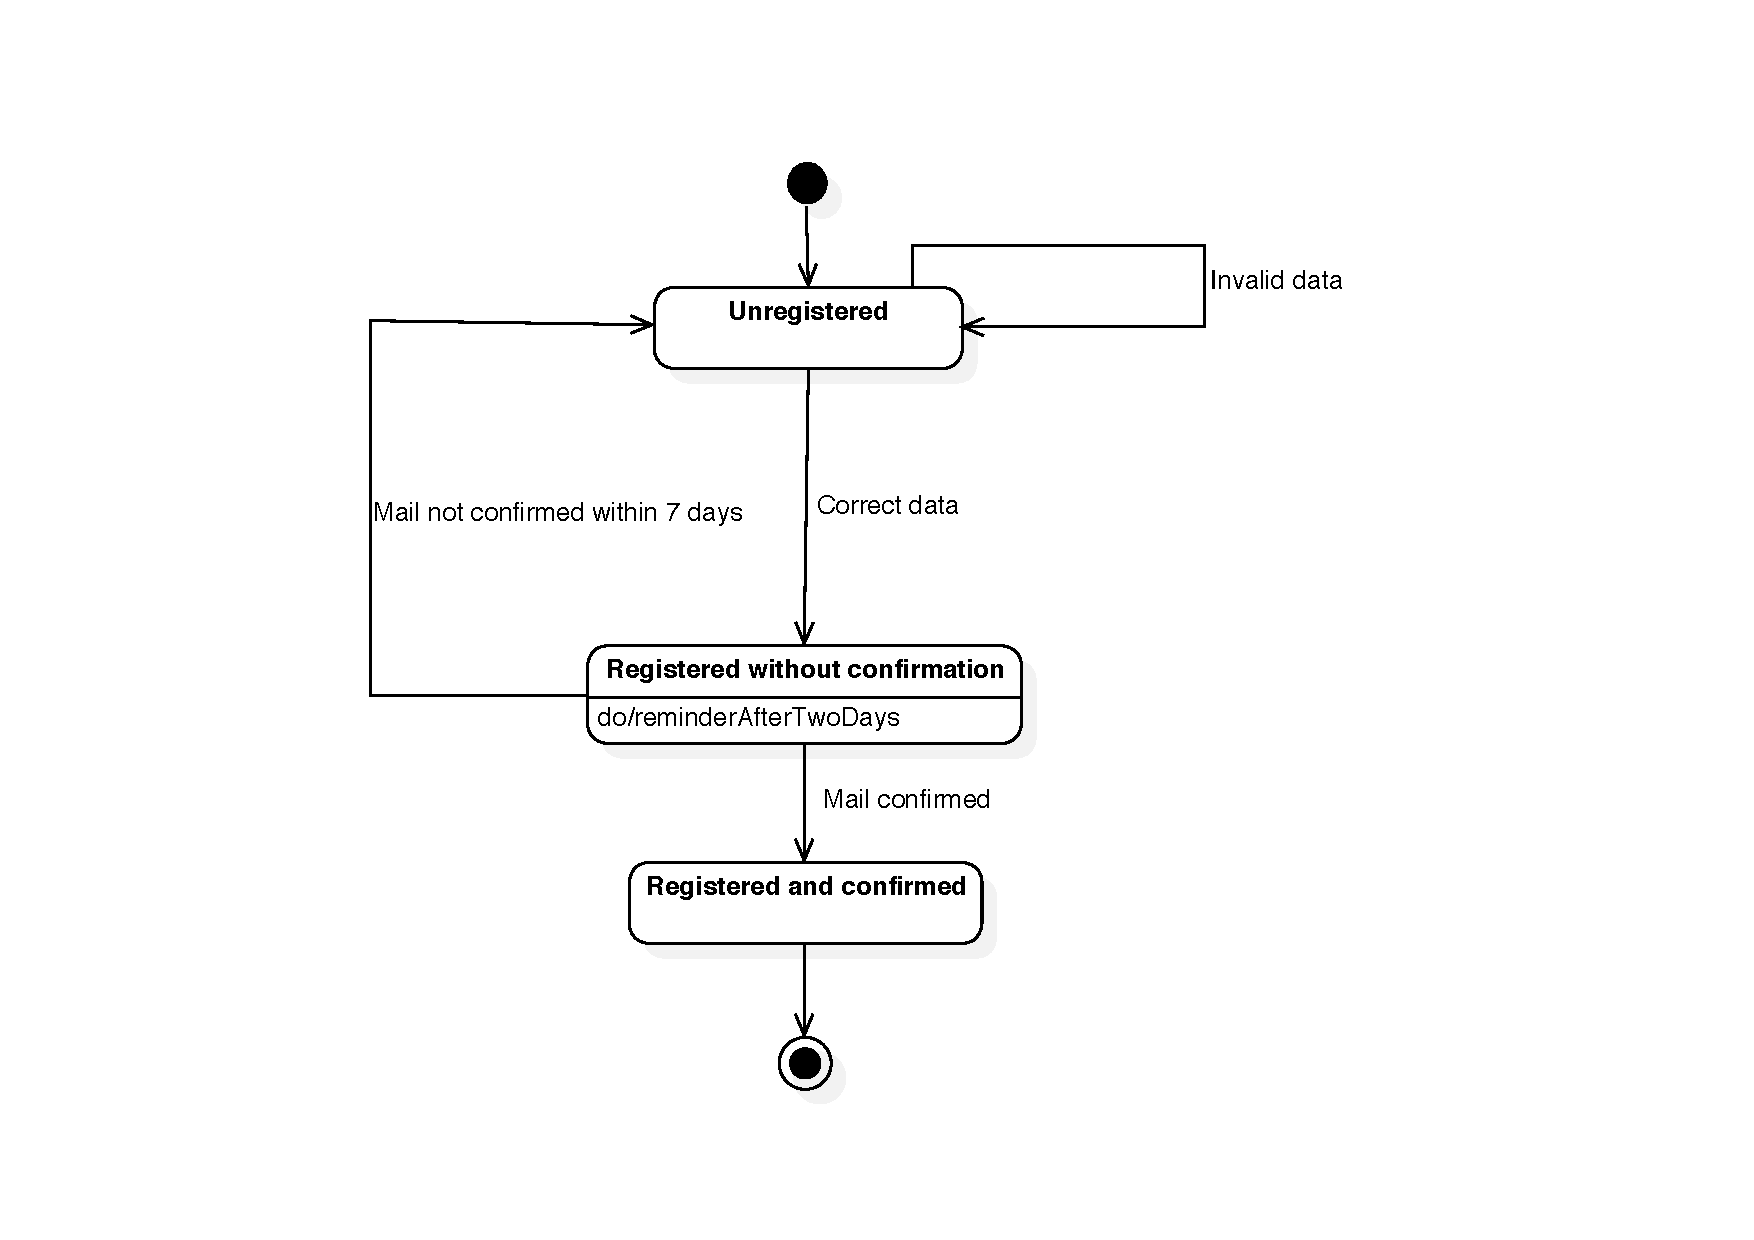
\includegraphics[width=0.7\textwidth]{diagrams/statechart_registration.pdf}
\caption{Statechart of the registration process.}
\label{fig:statechart-registration}
\end{center}
\end{figure}

\subsubsection{Associated functional requirements}

\begin{enumerate}
    \item On registration, the user can choose to register as a passenger or as a taxi driver.
    \item Passengers must provide the following information:
    \begin{itemize}
        \item e-mail address
        \item username
        \item password
        \item name
        \item surname
        \item address (optional filling)
        \item phone number (optional filling)
    \end{itemize}
    \item Taxi drivers must provide the following information:
    \begin{itemize}
        \item e-mail address
        \item username
        \item password
        \item name
        \item surname
        \item address
        \item phone number
        \item taxi license ID
        \item taxi number-plate
		\item number of passenger seats of the taxi
    \end{itemize}
    \item There mustn't be another user already subscribed with the same username or e-mail. \label{f-sameInfo}
    \item There mustn't be another taxi driver already subscribed with the same taxi license or taxi number plate. \label{f-sameTaxi}
    \item The username must match the regular expression\\``\texttt{[a-zA-Z][a-zA-Z0-9]\{2,20\}}''    \label{f-usrn}
    \item The system accepts a password that contains at least one number and one capital letter and that has a minimum length of eight characters.  \label{f-psw1}
    \item The system must ask for the password twice.
    \item The system accepts the password only if it is entered identically both times. \label{f-psw2}
    \item If the personal data treatment is not authorised, the subscription is canceled. \label{f-dataTreat}
    \item The system must allow the user to abort the registration process at any time.
    \item Email confirmation process:
    \begin{enumerate}
	    \item The subscription ends successfully when the user clicks on the link in the confirmation e-mail.
	    \item After two days without an answer, the systems sends another confirmation e-mail.
	    \item After seven days, the user's registration info are deleted and the user may re-try the registration process.  \label{f-confirm}
	\end{enumerate}
\end{enumerate}


\subsection{User login}
\label{user-login}
\subsubsection{Purpose}
Any subscribed user can login to use myTaxiService services.
The system requires the user to provide nickname and password, or e-mail and password, to log in correctly.

If the user doesn't remember his password, a new one is sent to the user's e-mail address. If the user clicks on the link in the e-mail, the password is reset and, as soon as he logs in, the system asks him to choose a new one. 



\subsubsection{Scenario 1}
Bob opens the home page of myTaxiService on the web and clicks on ``login''. 
he's asked to enter the nickname or the e-mail and the password. He doesn't recall his nickname, so he enters the registration e-mail and the password. He clicks on ``enter''. 
Everything is correct so he can access to the services as a logged user.

\subsubsection{Scenario 2}
Alice opens the home of myTaxiService page on web and clicks on ``login''.  
She is asked to enter the nickname or e-mail and the password.
She enters nickname and password and selects ``enter''. However, the entered password isn't correct so the system asks her to re-enter it. 
After some failed attempts she select ``password forgot''.
The system sends to her a new password via e-mail. She enters that one and the access is permitted, but before successfully ending the login the system requires her to change the password immediately. 
Alice changes her password and finally logs in to the services.

\begin{figure}
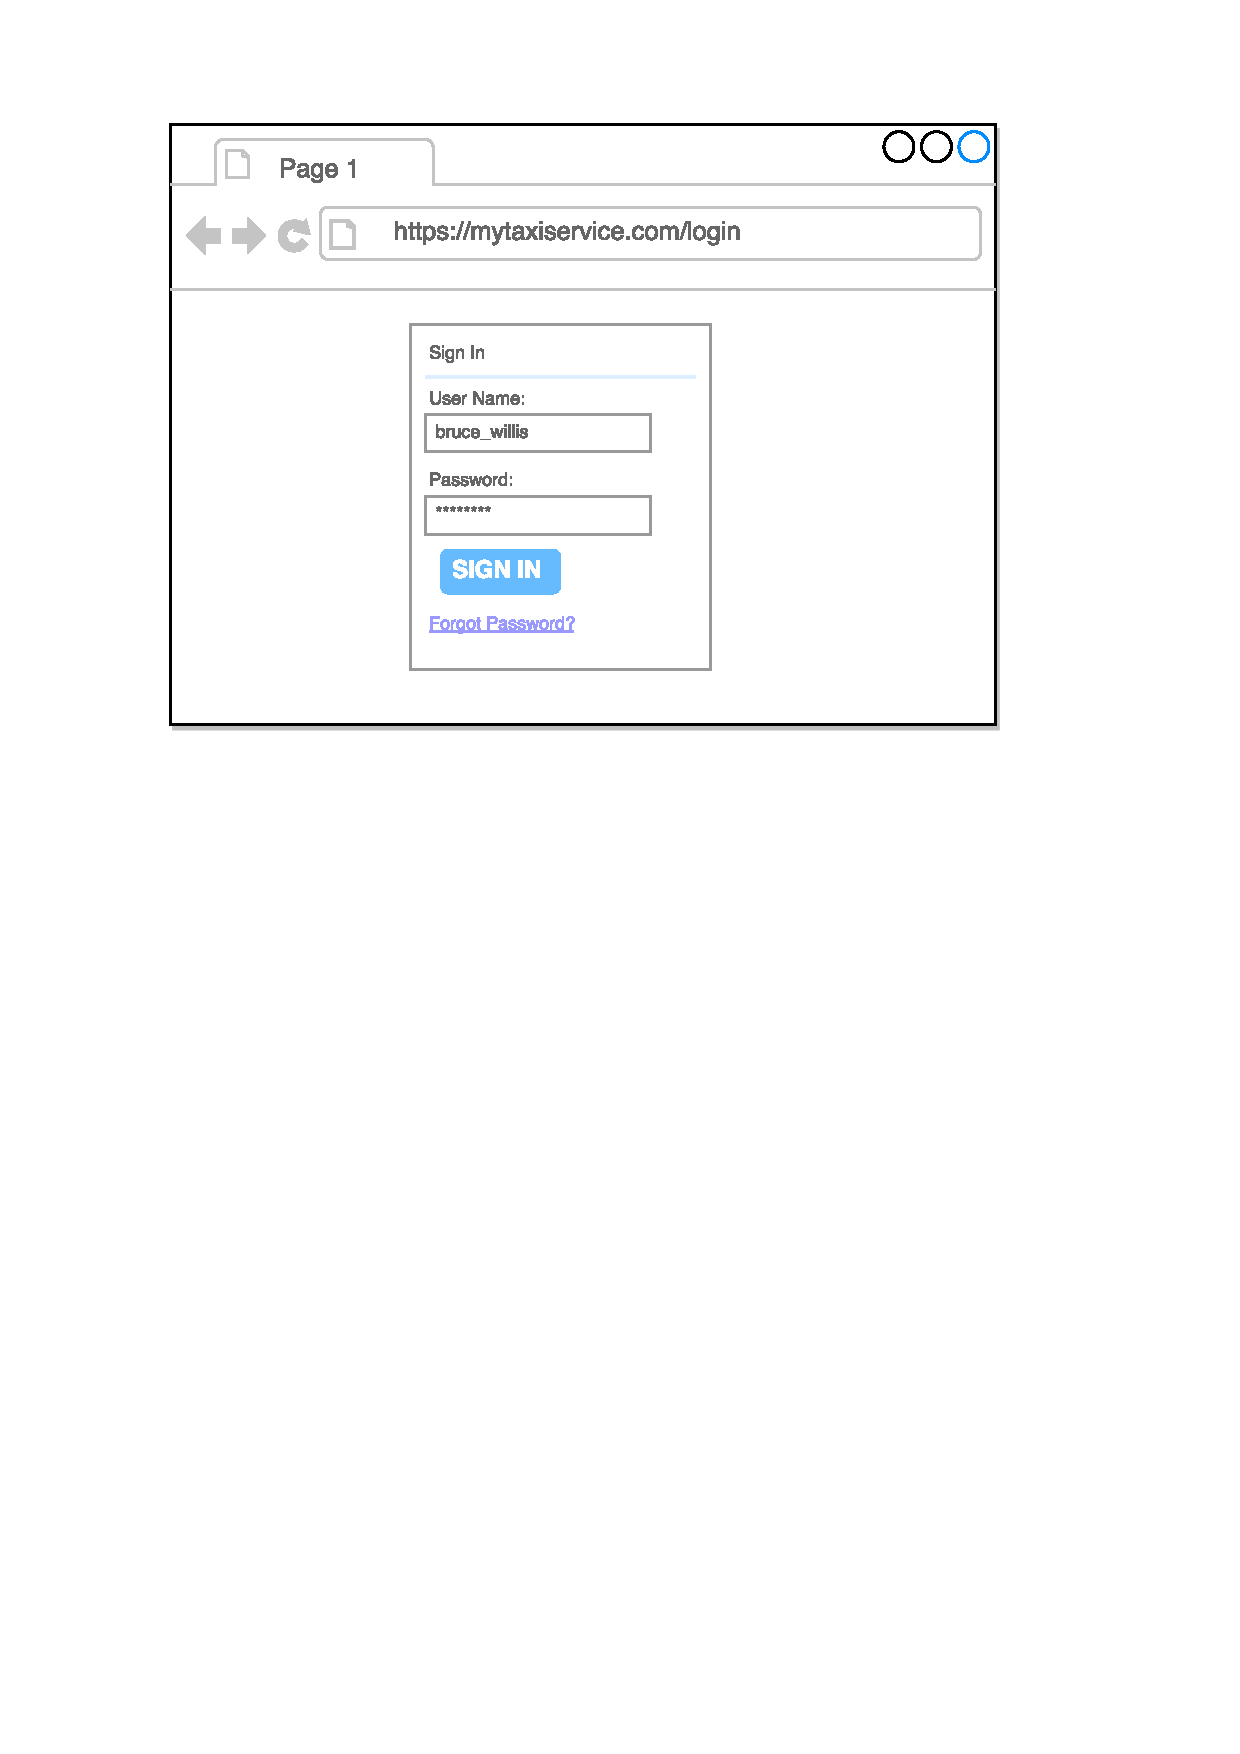
\includegraphics[width=\textwidth]{mockup/Login_browser.pdf}
\caption{Concept of the login webpage.}
\label{fig:mockup-login}
\end{figure}



\subsubsection{Use case}
The use case for user login is shown in~\autoref{usecase-login}.

\begin{table}
\begin{center}
\begin{tabular}{| l | p{0.6\textwidth} |}
\hline
Actor & Registered passenger or taxi driver \\
\hline
Goal & Goal ~\ref{g-login}
\\
\hline
Input condition & The user, already registered, chooses to login.  \\
\hline
Event Flow & \begin{enumerate}
	\item The user selects ``login''.
	\item The login page is shown. \label{load-login}
	\item The user enters his/her credentials.
	\end{enumerate}
\\
\hline
Output condition & The system tells the user that he/she has been successfully logged in.
It is loaded the main page where the user can choose one of the myTaxiService options. \\
\hline

Exception & If the username/e-mail or password entered are wrong, the system notifies the user and the login page is reloaded (step~\ref{load-login} of Event Flow): the login has failed. 

	
 \\
\hline
\end{tabular}
\end{center}
\caption{Use case for user login.}
\label{usecase-login}
\end{table}





\subsubsection{Response sequence}
The response sequence is illustrated in figure \ref{fig:sequence-login}.
\begin{figure}
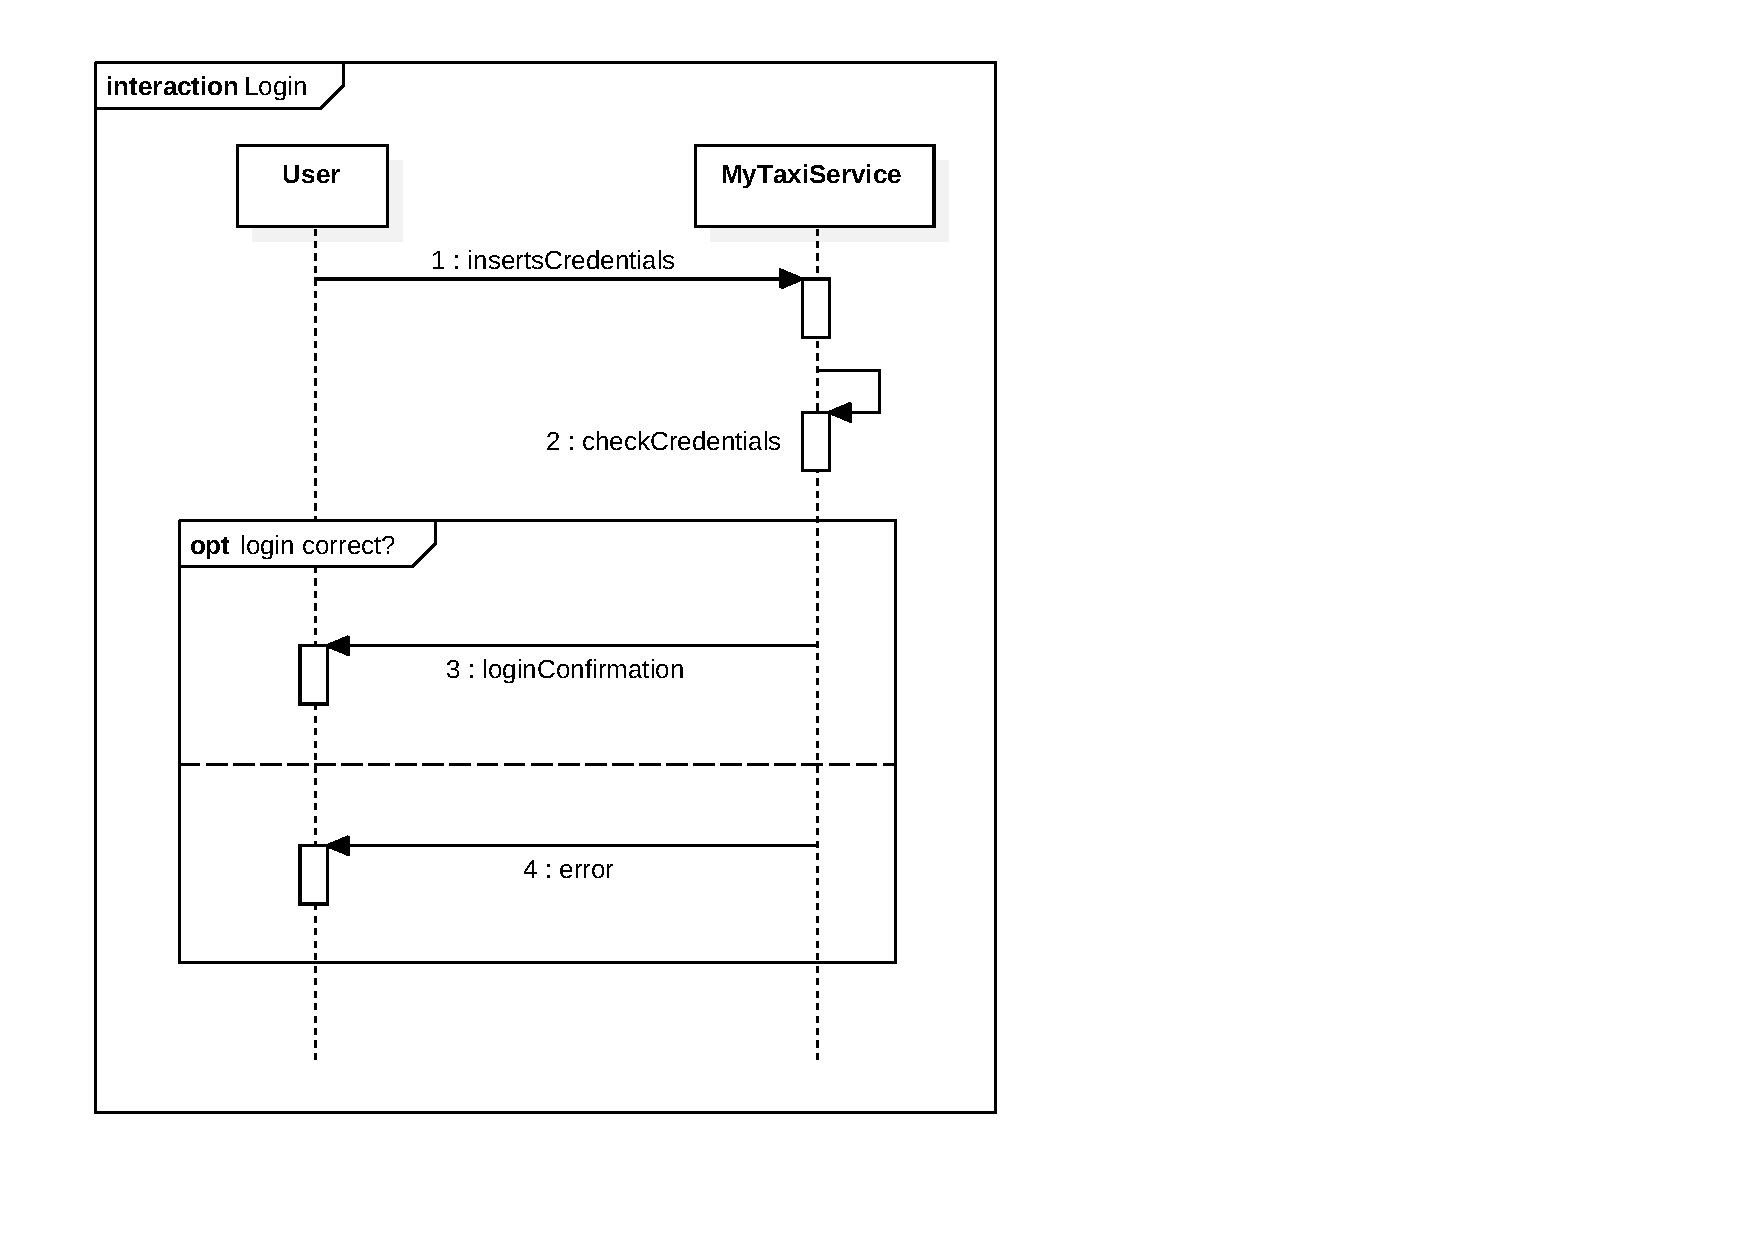
\includegraphics[width=\textwidth]{diagrams/sequence_login.pdf}
\caption{Sequence diagram of a user login.}
\label{fig:sequence-login}
\end{figure}

\subsubsection{Associated functional requirements}
\begin{enumerate}
    \item In order to log in, the user must insert either a nickname, or the registration e-mail, but not both.
    \item On login, the system must grant to the user access to his/her account if and only if the following conditions are met:
    \begin{enumerate} 
    	\item The inserted nickname corresponds to a username of an existing user, or the inserted e-mail corresponds to the registration e-mail of an existing user.
	\item The inserted password is the same of that of the user identified above.
    \end{enumerate}
    \item The system sends an e-mail after the ``password forgot'' button is selected.
    \item The system reset the user's password only after the link on e-mail is clicked.
    \item If the password entered is wrong a new attempt can be made only 10 seconds later.
  
\end{enumerate}

\subsection{Standard taxi call}
\label{standard-call}
\subsubsection{Purpose}

Any subscribed passenger shall be able to request a taxi either through the web application or the mobile app.
After the request, the passenger is informed by the system about the waiting time and the code of the incoming taxi.

Requests shall be forwarded to available and active taxi drivers in the same zone of the passengers. Taxi drivers shall be able to accept or reject an incoming request.

\subsubsection{Scenario 1}
Alice needs a taxi. She opens the myTaxiService mobile app on her phone, and selects ``Call a taxi''. She authorizes the application to access her GPS data, checks on the map that her position is correct and confirms the request.

The system forwards the request to Bob, the first taxi driver in Alice's taxi zone. Bob decides to accept the call: a map of Alice's position gets displayed on Bob's phone and the navigator starts.

Bob's position is transmitted from his phone to the system, which computes the ETA for the incoming taxi and shows it to Alice. Bob arrives and picks Alice up. Then he confirms that the passenger is on board.

When the ride is over, Bob taps on ``Finish ride'' so that the system knows that Bob is ready for another ride.

\subsubsection{Scenario 2}
Luke needs a taxi. He requests it and the request is forwarded to the first taxi driver in queue, Chewbacca. Chewbacca decides to reject the incoming request, so the system puts him at the bottom of the queue.

Luke's request gets forwarded to the new first taxi driver in queue, Han Solo. Han accepts the request and comes to pick up Luke.

\subsubsection{Scenario 3}
Luke, Leila and Obi-Wan need a taxi. Luke has myTaxiService app on his phone so he opens it and selects ``Call a taxi''. He checks that position is correct, he enters three as number of seats required and confirms the request.

Luke's request gets forwarded to the first taxi driver in queue, Han Solo, that accepts the request and comes to pick up the group of friends.


\begin{figure}
\begin{center}
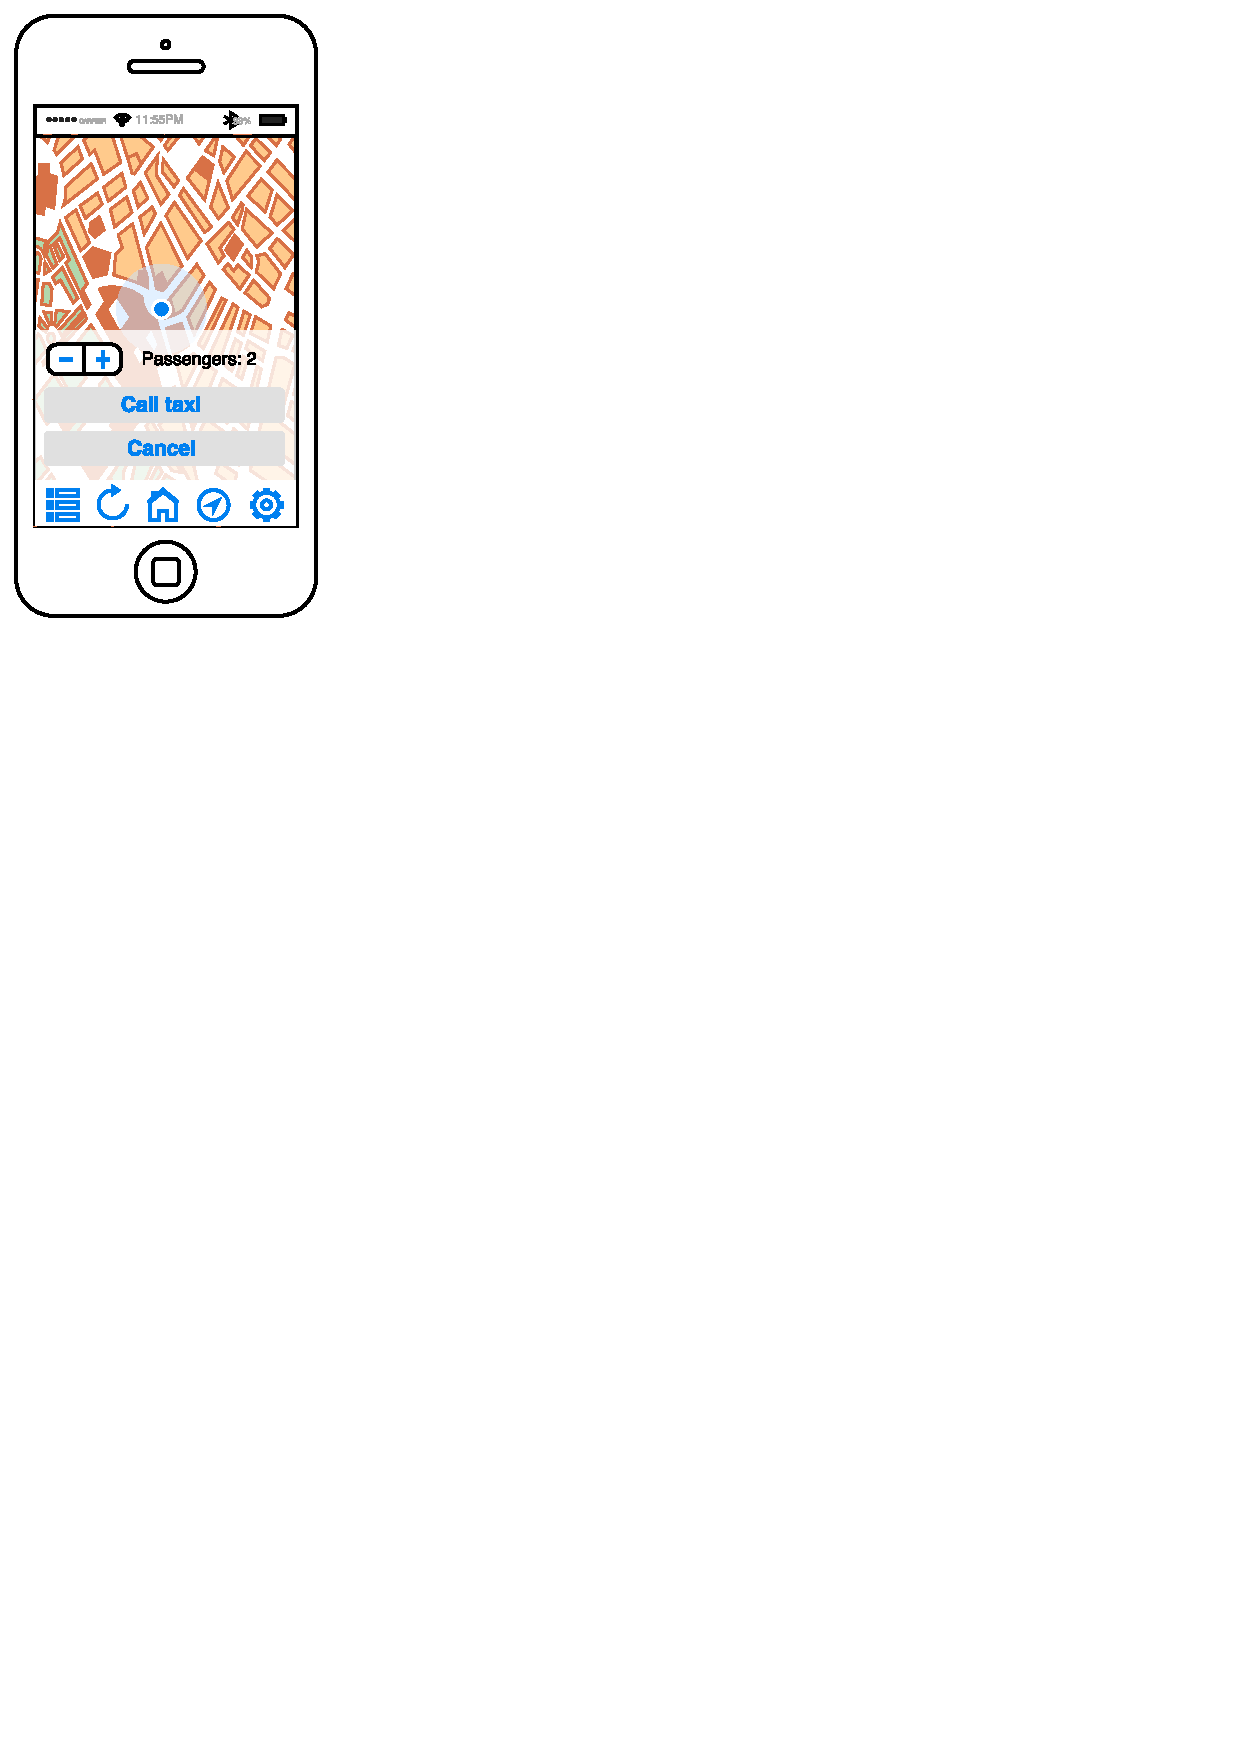
\includegraphics[width=0.4\textwidth]{mockup/TaxiCall.pdf}
\caption{Concept of the taxi call interface.}
\label{fig:mockup-taxicall}
\end{center}
\end{figure}

\subsubsection{Use case}
The use case for a taxi call is shown in~\autoref{usecase-taxicall}.

\begin{table}
\begin{center}
\begin{tabular}{| l | p{0.6\textwidth} |}
\hline
Actor & Passenger \\
\hline
Goal & Goal~\ref{g-taxicall}
\\
\hline
Input condition & Passenger is already logged in and requests a taxi.  \\
\hline
Event Flow & \begin{enumerate}
	\item The passenger requests a taxi through the client.
	\item The request gets forwarded to the first taxi in the queue of the same taxi zone of the user.
	\item The taxi driver can either accept or deny the request; if he denies it, the request is forwarded to the next taxi driver in the queue, and so on.
	\item Finally the request gets accepted by a taxi driver.
	\item The passenger gets notified that a taxi driver accepted his request and is given the ETA of the incoming taxi.
	\item When the taxi driver meets the passenger, he/she signals that the passenger is on board.
\end{enumerate}
\\
\hline
Output condition & The driver confirms that the passenger is aboard. \\
\hline
Exception & No taxi is available in the passenger's zone. \\
\hline
\end{tabular}
\end{center}
\caption{Use case for a standard taxi call.}
\label{usecase-taxicall}
\end{table}

\subsubsection{Response sequence}
The response sequence is illustrated in figures \ref{fig:sequence-taxicall} and \ref{fig:sequence-taxicall-refused}.

\begin{figure}
	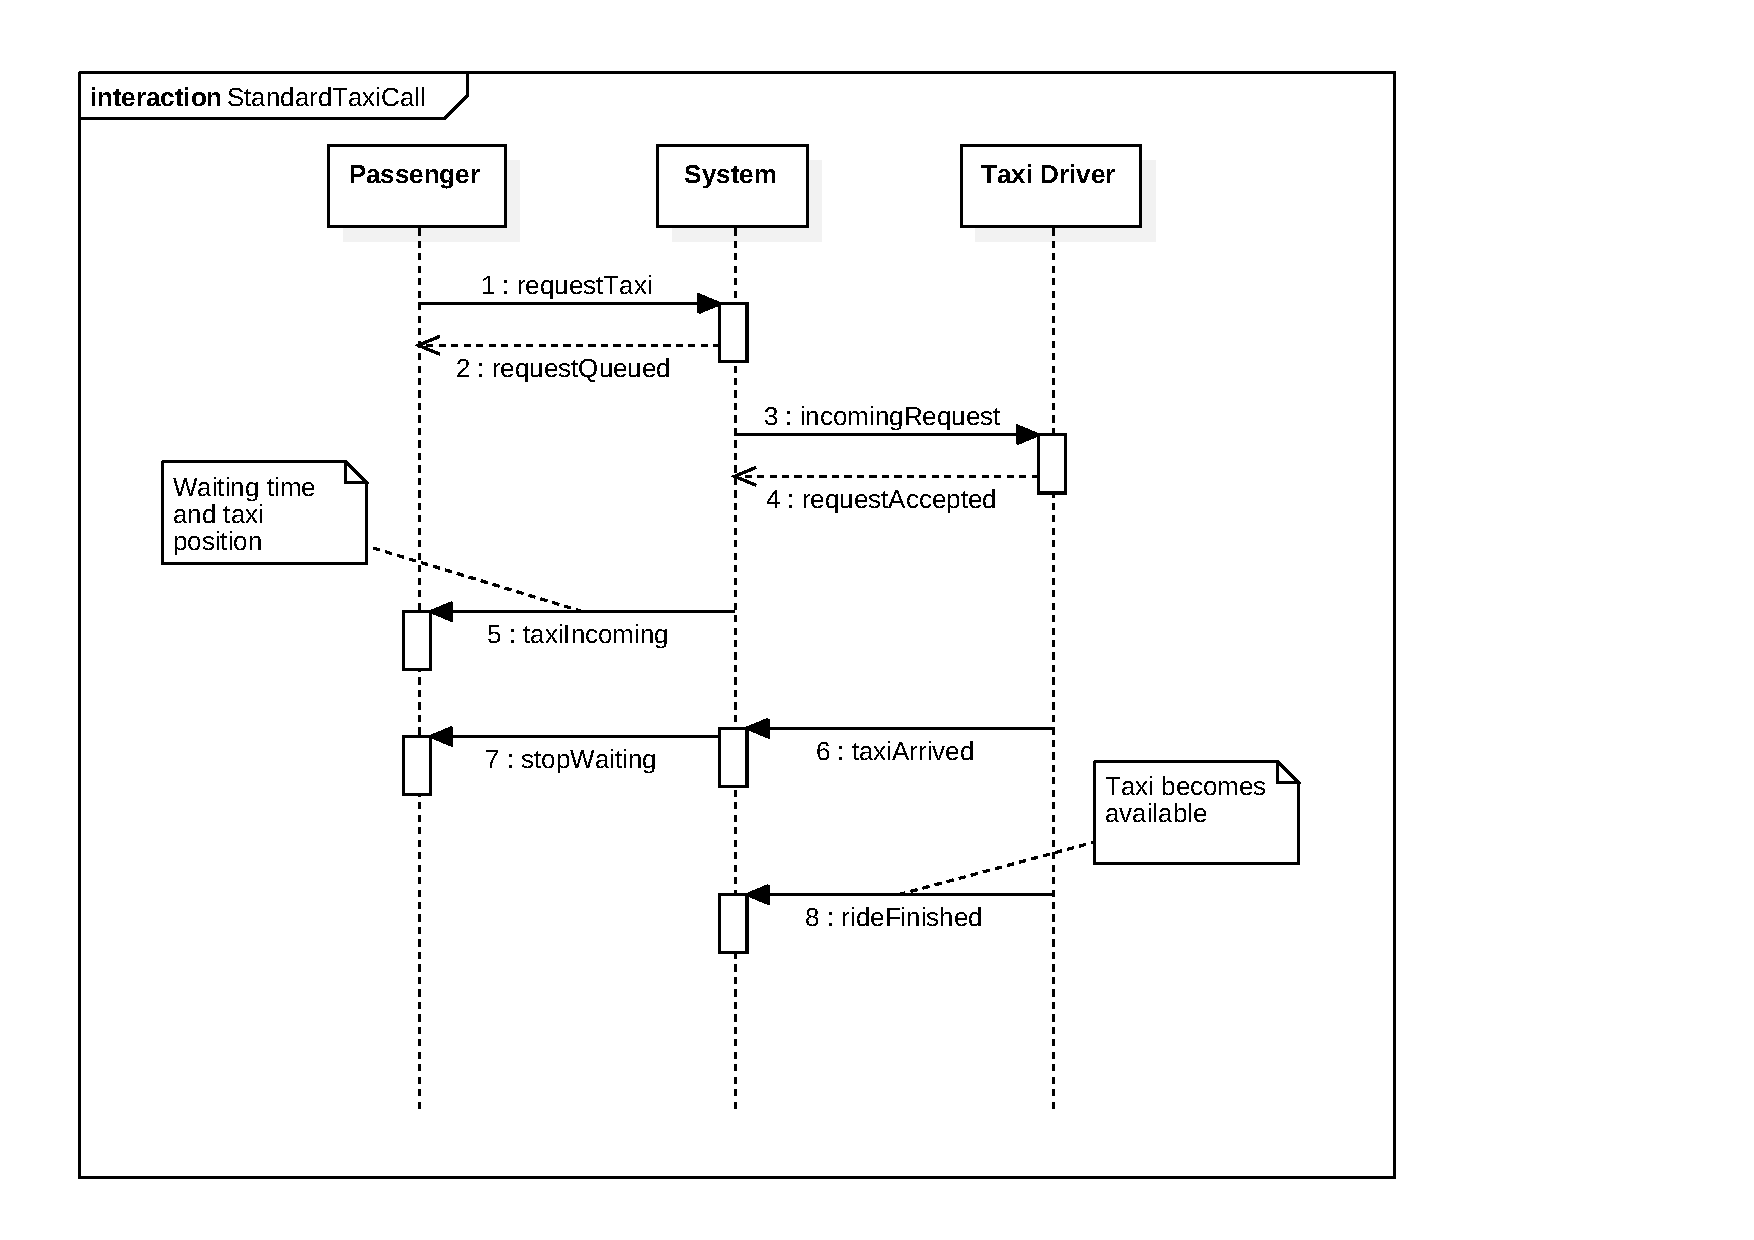
\includegraphics[width=\textwidth]{diagrams/sequence_taxicall.pdf}
	\caption{Sequence diagram of a successful taxi call, picked up by the first taxi driver called by the system.}
	\label{fig:sequence-taxicall}
\end{figure}

\begin{figure}
	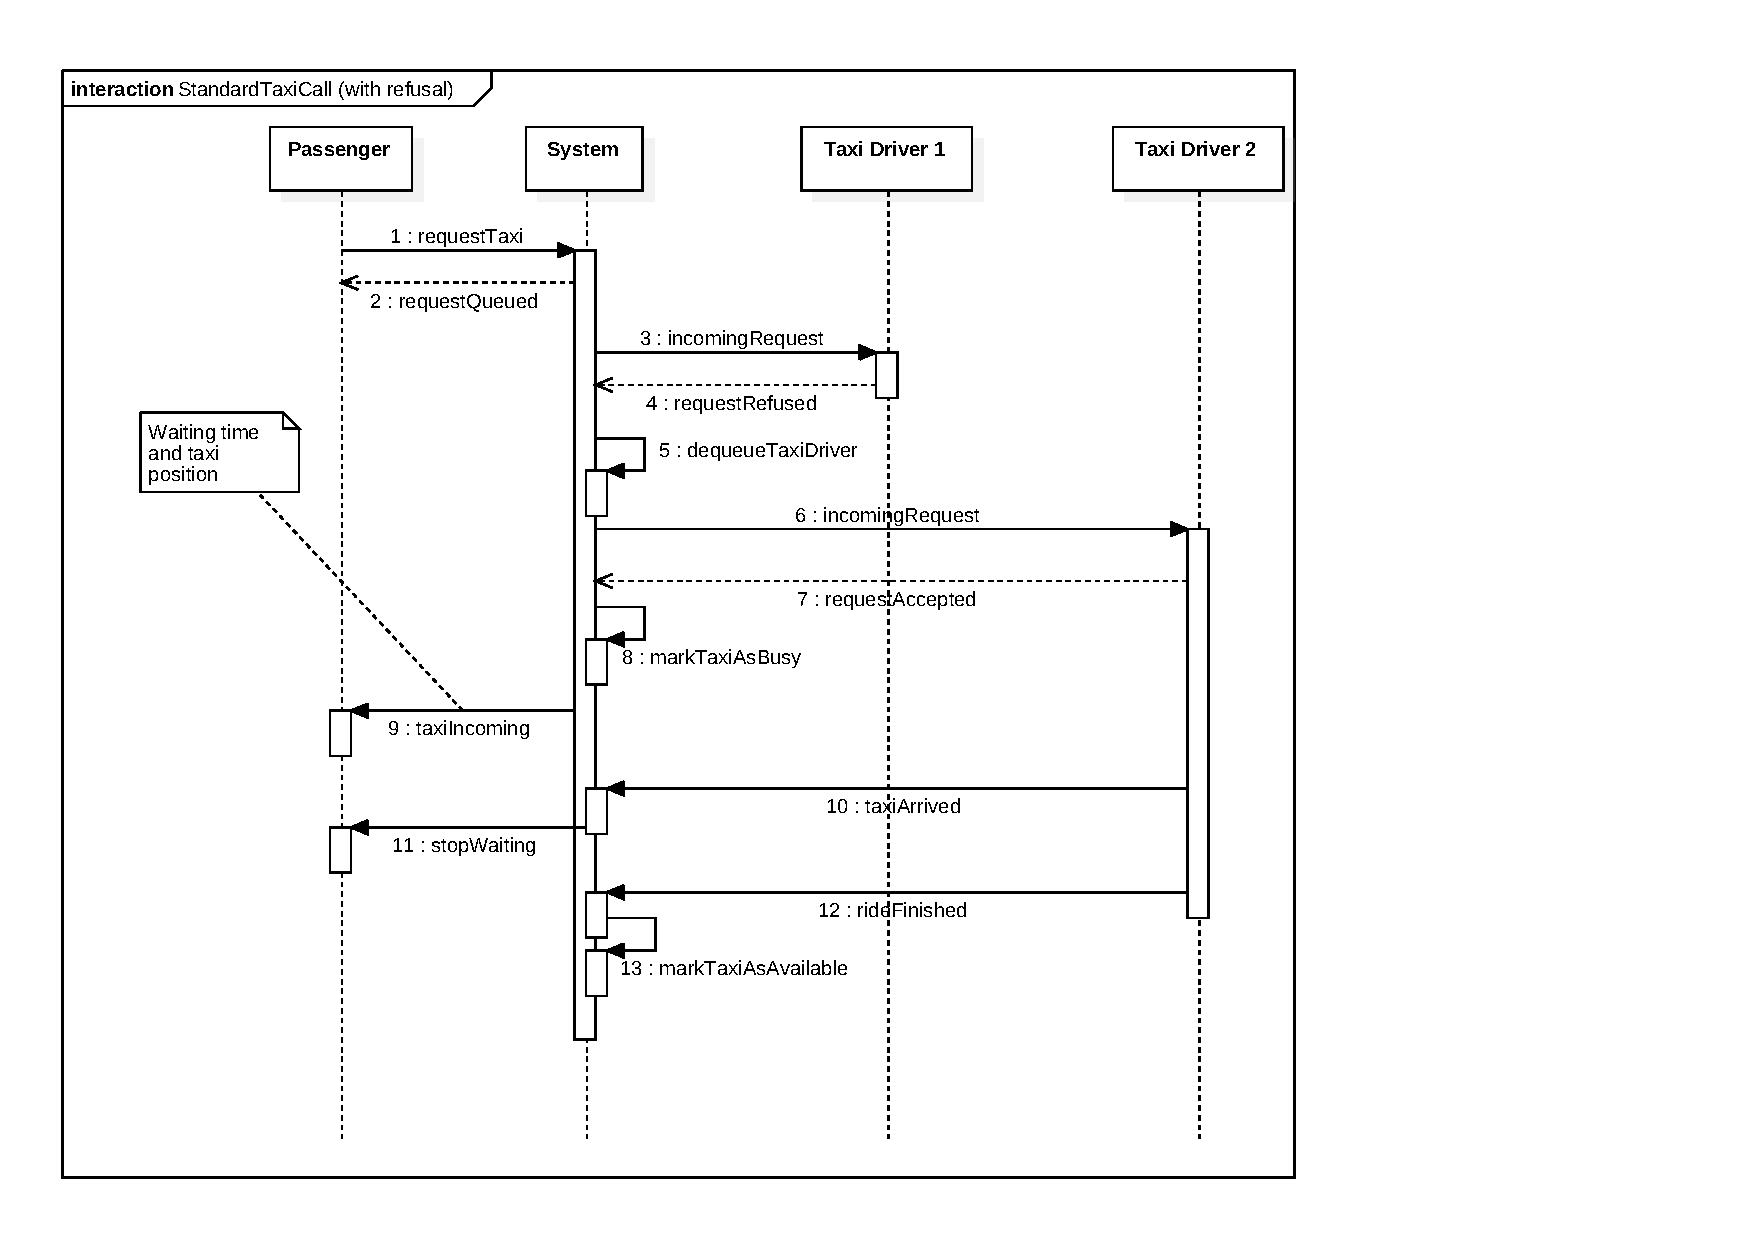
\includegraphics[width=\textwidth]{diagrams/sequence_taxicall_refused.pdf}
	\caption{Sequence diagram of a taxi call when the first taxi driver to receive the request refuses the call and the second one accepts it.}
	\label{fig:sequence-taxicall-refused}
\end{figure}

\subsubsection{Associated functional requirements}
\begin{enumerate}
	\item The system must localize the passenger before he or she makes a taxi request.
	\begin{enumerate}
		\item (App) If GPS info is available and the passenger can be tracked within a radius of 50 m, then the passenger is presented with the option of using the current GPS position.
		\item (App) If GPS info is not available or the precision is less than 50 m, then the app requests the passenger to insert a valid address. Then the address is shown on a map and the passenger can confirm its position.
		\item (Web) In the web application the user is always requested to insert a valid address. Then the address is shown on a map and the user can confirm its position.
	\end{enumerate}

	\item When the system knows the passenger's position, it asks the number of seats required in the taxi.
	\item Once the system knows the number of seats required, it presents the passenger the option to request a taxi.
	\item The system must ask the passenger for confirmation before delivering the taxi request.
	\item After the passenger's confirmation of a taxi request, the request is delivered to the first taxi with a sufficient number of seatss in the queue for the taxi zone in which the user is located.
	\item Taxi requests are forwarded only to active taxi drivers which are located in the same taxi zone, who are not currently busy.
	\item Taxi requests are processed in order of arrival.
	\item If there's no taxi driver in the passenger's taxi zone, the request is refused and en error message is displayed to the passenger.
	\item When a taxi driver receives a request, the mobile application shows a notification and emits a sound.
	\item When receiving a request, the taxi driver is presented with the possibility of accepting or denying it.
	\item After having accepted a request, the taxi driver is automatically marked as ``busy''.
	\item After having accepted a request, the mobile application shows to the taxi driver a map with the location of the passenger, and automatically starts navigation instructions on the app preferred by the taxi driver (Google Maps, Waze, TomTom, etc.).
	\item After the taxi request is accepted, the app shows the passenger a map with the current position of the incoming taxi.
	\item After the taxi request is accepted, the passenger is informed about the ETA for the incoming taxi.
	\item The ETA for the incoming taxi is fetched from the server every 90 s.
	\item The ETA for the incoming taxi is computed by the system considering the distance from the taxi to the passenger and the current traffic conditions.
	\item When the taxi is within 20 m from the passenger, the app asks the taxi driver to confirm that the passenger is aboard.
	\item When the taxi driver confirms that the passenger is aboard, the taxi request is marked as fulfilled and the system stops showing the waiting time to the passenger.
	\item The system must prevent the passenger to call a taxi while he/she is already waiting for one.
	\item The system must prevent the passenger to call a taxi while he/she is already traveling in a taxi.
\end{enumerate}


\subsection{Ride request notification to the taxi driver}
\label{driver-notification}
\subsubsection{Purpose}

After a taxi driver has informed the system about his/her availability (section~\ref{taxi-availability})
he/she will be able to receive ride request notifications. The taxi driver receives the notification on his/her cell phone and has one minute to accept or reject the request. If after one minute the request is not answered, the system will consider the request as refused.

\subsubsection{Scenario 1}
Travis, who suffers from chronic insomnia, every night waits in his taxi for an incoming request. When a user requests a taxi, the system processes the request and decides which taxi driver to send.

For a new incoming request, the system chooses Travis, who is on the top of the queue and in the same taxi zone of the passenger. The system sends him a notification on his mobile app. Travis reads the message which reports location and time of the meeting and decides to accept the request pushing the appropriate button on the display.

The system acknowledges the decision and waits for Travis to notify that the passenger is on board (last part of~\ref{standard-call}).

\subsubsection{Scenario 2}
The system receives a new incoming request from a user and selects Frank Martin as designated taxi driver (section~\ref{taxi-availability}).
The system sends him a notification and waits for the reply.

Frank has just finished a very demanding ride, so he decides to refuse the request using the interface of the app. The system receives Frank's decision and looks for another available taxi on the same taxi area.

\begin{figure}
\begin{center}
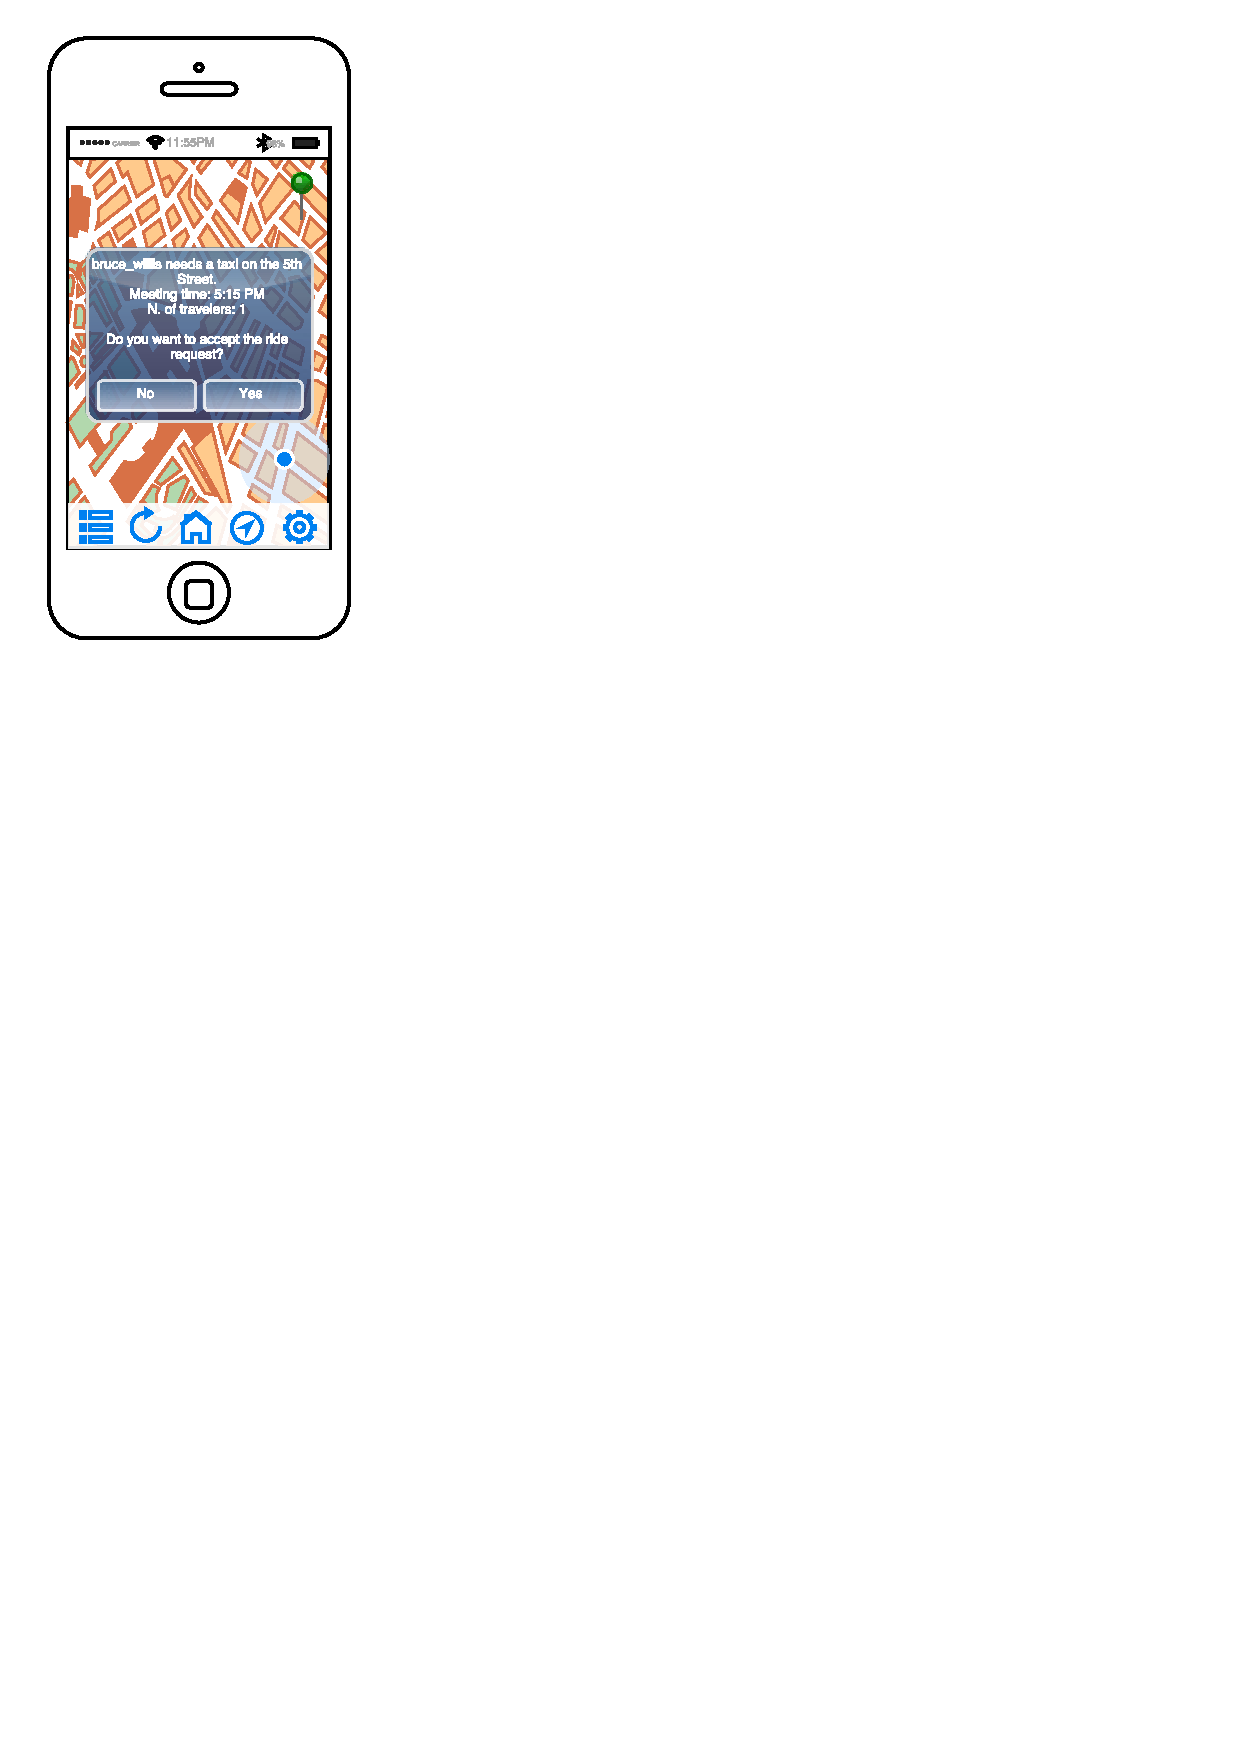
\includegraphics[width=0.4\textwidth]{mockup/RideRequest.pdf}
\caption{Concept of the ride request notification.}
\label{fig:mockup-riderequest}
\end{center}
\end{figure}

\subsubsection{Use case}
The use case for a driver notification is shown in~\autoref{usecase-drivernotification}.

\begin{table}
\begin{center}
\begin{tabular}{| l | p{0.6\textwidth} |}
\hline
Actor & Taxi driver \\
\hline
Goal & Goal~\ref{g-notify}
\\
\hline
Input condition & The system informs the taxi driver about a new request.  \\
\hline
Event Flow & \begin{enumerate}
	\item The system informs the taxi driver about a new request, specifying time and location of the ride
	\item The taxi driver sees the information on his cell phone and chooses whether to accept or to refuse the request
	\item If after a minute the taxi driver has not sent the response, the system considers the request refused
	\item If the request is accepted,  the system dequeues the taxi and marks it as busy, otherwise it sends the request to the next taxi
	\item When someone has accepted, the system notifies it to the passenger specifying the arrival time of the taxi
	\end{enumerate}
\\
\hline
Output condition & The system informs the passenger about the estimated time arrival of the taxi. \\
\hline
Exception & No taxi replies the request. \\
\hline
\end{tabular}
\end{center}
\caption{Use case for driver notification.}
\label{usecase-drivernotification}
\end{table}

\subsubsection{Response sequence}
The use case associated to the response sequence is shown in figure~\ref{fig:sequence-taxicall-refused}.

\subsubsection{Associated functional requirements}
\begin{enumerate}
\item The app must show the request notification to the taxi driver.
\item The system allows the taxi driver to accept or decline the request using the app.
\item The app must produce sounds or visual notifications as the taxi driver has chosen.
\item The system must use timeouts in order to prevent infinite pending requests.
\item The system has to provide the taxi driver with information about the time and place of the meeting with the passenger.
\item The system gives to the taxi driver one minute to reply. Else, the request is automatically refused.
\end{enumerate}


\subsection{Taxi availability handling}
\label{taxi-availability}
\subsubsection{Purpose}

When a taxi driver is ready for a ride, he/she shall be able to notify the system using his mobile phone. With the app he/she can change his status from "not in service" to "in service".

When the system receives the status update from the taxi driver, it inserts him/her in the right queue for his/her taxi zone using the information from the taxi GPS if the new status is "in service", or it removes him/her from the queue if the new status is "not in service".

After a ride, a taxi driver has to notify, using the dedicated section of the app, that the ride is over. The system shall reinsert the taxi into the right queue.
%TODO define FIFO

The queues are FIFO and when a taxi driver refuses a ride, the system moves the taxi to the bottom of the same queue.

When a taxi driver accepts a ride, the system marks the taxi as busy and removes it from the top of the queue.

\subsubsection{Scenario 1}
Ernie gets in his taxi, ready to start his working day. He takes out his phone from his pocket and after logging in he changes his status in "in service".

The system acquires the changing and retrieves the GPS position of Ernie's taxi. It analyses the data and puts the taxi in the right queue.

After thirty minutes the system has an incoming request from the Ernie's zone. The first taxi on the top of the queue is Ernie's. The system sends a notification to Ernie and waits for a reply.

Ernie receives the request and accepts the meeting. The system pops Ernie from the top of the queue and marks it as busy.

When Ernie accomplishes the ride, he notifies the system, which retrieves the new GPS position and inserts Ernie's in the queue.

\subsubsection{Use case}
The use case for a taxi availability handling is shown in~\autoref{usecase-taxiavailability}.

\begin{table}
\begin{center}
\begin{tabular}{| l | p{0.6\textwidth} |}
\hline
Actor & Taxi driver \\
\hline
Goal & Goal~\ref{g-notify}
\\
\hline
Input condition & Taxi drivers are logged in and change his status to "in service".  \\
\hline
Event Flow & \begin{enumerate}
	\item The taxi driver changes his status to "in service"
	\item The system enqueues the taxi in the right queue using GPS informations
	\item A new request incomes
	\item The system chooses the first taxi in the queue and sends the request for a ride
	\item The taxi driver can either accept or deny the request; if he denies it, the request is forwarded to the next taxi driver in the queue, and so on.
	\item When a taxi driver accepts the request, the system dequeues it and marks it as busy
	\item The taxi driver drives to the location
	\item The taxi driver notifies that the passenger is on board
	\item When the ride is completed, the taxi driver notifies it to the system
	\item The system enqueues the taxi in the right queue using GPS informations
	\item The taxi driver changes his status to "not in service"
	\item The system dequeues the taxi
\end{enumerate}
\\
\hline
Output condition & The driver changes his status to "not in service". \\
\hline
Exception & No taxi is available in the passenger's zone. \\
\hline
\end{tabular}
\end{center}
\caption{Use case for taxi availability handling.}
\label{usecase-taxiavailability}
\end{table}

\subsubsection{Response sequence}
The response sequence associated with this functionality is shown in figure~\ref{fig:taxi_availability}.
\begin{figure}
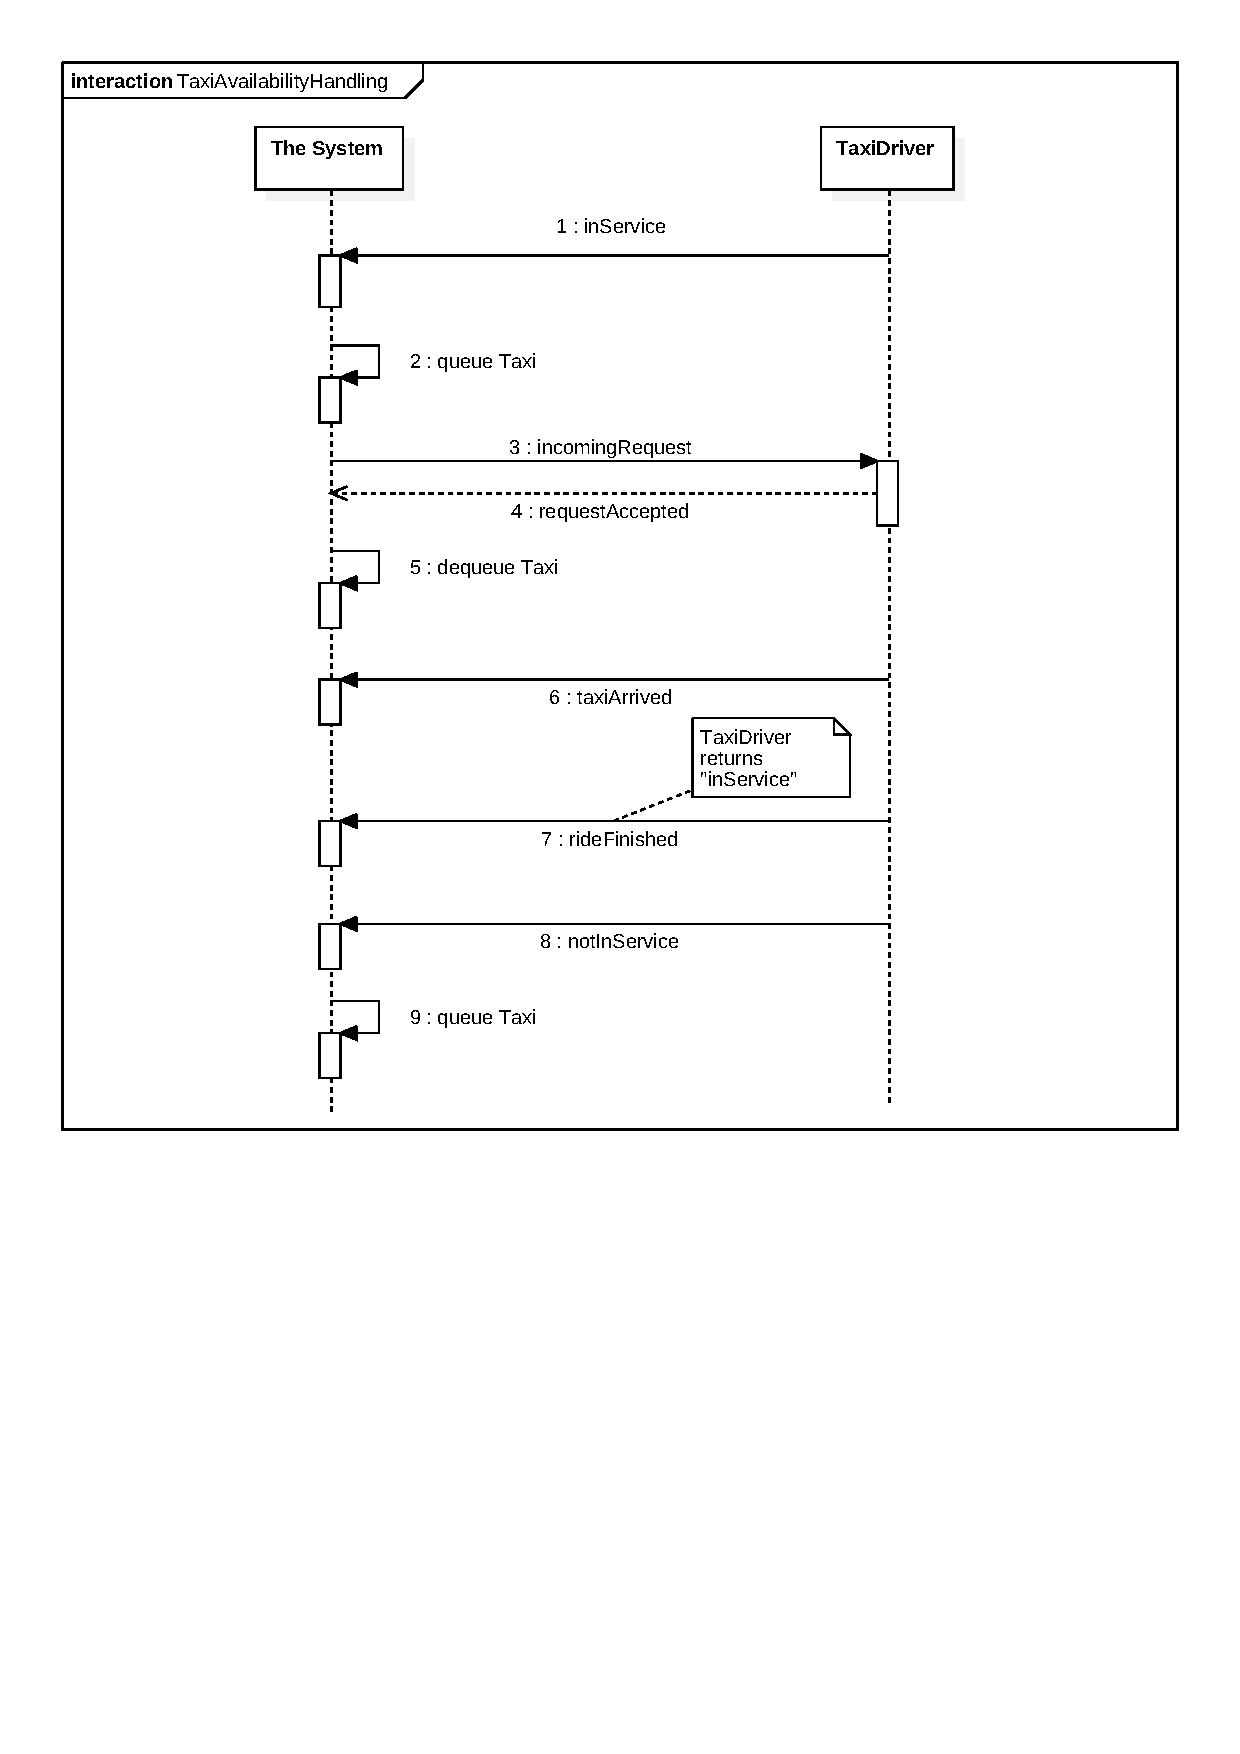
\includegraphics[width=\textwidth]{diagrams/taxi_availability_handling.pdf}
\caption{Sequence diagram of an accepted taxi call.}
\label{fig:taxi_availability}
\end{figure}

\subsubsection{Associated functional requirements}
\begin{enumerate}
\item The system knows the information about the GPS installed on the taxi.
\item The mobile app has to offer to the taxi driver the "change status" function and the "ride complete" function.
\item The system must notify the taxi when a request is incoming.
\item The system inserts the taxi in the right queue and changes it if the taxi changes area.
\item For every new request, the system chooses the taxi driver on the top of the queue.
\item The taxi driver has to reply in one minute to the request, else the ride is automatically refused.
\item The system manages the queues using the FIFO policy.
\item When busy, the taxi driver is presented by the mobile application with the option to end the ride.
\item When the taxi driver ends the ride, he or she is marked as available and gets re-inserted in the taxi queue of the taxi zone where he or she is located.
\end{enumerate}


\subsection{Taxi reservation}
\subsubsection{Purpose}

Any subscribed passenger shall be able to reserve a taxi for a ride at a predefined time. The passenger has to specify in advance the origin and the destination of the ride, along with the starting date and time.

\subsubsection{Response sequence}
% Sequence diagrams and use cases

\subsubsection{Associated functional requirements}
\begin{enumerate}
\item The system presents the passenger with the option to reserve a taxi.
\item The system asks the passenger the origin and the destination of the ride.
\item Origin and destination must be valid addresses.
\item If GPS info is present and accurate within 50 m, the passenger can specify "current position" as the destination of the ride.
\item The system asks passenger for the date and time of the ride.
\item The system lets the passenger enter only valid dates and times.
\item The system lets the passenger reserve a taxi from 48 hours to 2 hours before the actual ride time.
\item 10 minutes before the specified arriving time, the system allocates a taxi for the passenger by putting a request in the queue as described in subsection~\ref{standard-call}.
\item After the request is accepted, the passenger gets notified with the ETA of the incoming taxi along with its position.
\end{enumerate}

\subsection{Ride sharing}
\label{ride-sharing}
\subsubsection{Purpose}

Every subscribed passenger shall be able to activate the ride sharing function in the mobile app or in the web interface. When this mode is enabled, the passenger has to provide the system also with a destination for the ride.

The system, before allocating a taxi, inserts the pending ride in the set of shared rides and tries to identify possible sharing solutions.
With an adequate algorithm it can propose every feasible sharing solution to the user.

The first user who reserves a taxi is called the ``owner'' of the ride.
The passenger can choose to join one of the pending rides or to refuse the proposal, becoming the owner of a new ride.

In the first case the system informs the owner of the ride. The new passenger has to go to the meeting point with the owner of the ride in time. If he/she is not able to do that the taxi does not wait for him/her.

In the second case the system allocates the taxi (\ref{taxi-availability}) and applies the standard procedure (\ref{standard-call}).  The user becomes the owner of the ride.
If there is another passenger willing to share the same ride, the system allows it and redirects this last user to the meeting point with the owner, who is informed as well as the taxi driver.

\subsubsection{Scenario 1}
Batman needs a taxi and decides to enable the sharing mode on his cell phone. The app also asks Batman for the destination of his travel.

When Batman submits the form, the system matches the path of Batman's ride with every pending ride started from Batman's area. It finds only one compatible ride and sends it to Batman.

Batman finds that it is Joker's pending ride and refuses to share the ride.
So, the system allocates a new taxi.

A new user, Robin, is in Batman's area and needs a taxi. He decides to enable the sharing function and the system proposes him Batman's and Joker's rides.
He chooses Batman's: the system, which has already communicated location and time to Robin, notifies Batman and the taxi driver that there is an additional passenger.

When the taxi arrives, the taxi driver confirms from his mobile app how many passengers he has picked up.

\subsubsection{Use case}
The use case for a ride sharing is shown in~\autoref{usecase-ridesharing}.

\begin{table}
\begin{center}
\begin{tabular}{| l | p{0.6\textwidth} |}
\hline
Actor & Taxi driver and Multiple Passengers \\
\hline
Goal & Goal~\ref{g-share}
\\
\hline
Input condition & The user enables the sharing option from his mobile phone or from the web interface.  \\
\hline
Event Flow &
\begin{enumerate}
	\item The passenger enables the sharing option.
	\item The passenger enters a destionation.
	\item The system computes the feasible shared rides and proposes them to the passenger.
	\item The passenger can accept one of the sharing options or refuse all of them.
	\item If the passenger refuses, the system executes the standard taxi call \ref{standard-call}, otherwise it notifies the owner of the ride and the taxi driver.
\end{enumerate}
\\
\hline
Output condition & The system informs the owner of the ride and the taxi driver that the ride will be shared. \\
\hline
Exception & No taxi available in the area. \\
\hline
\end{tabular}
\end{center}
\caption{Use case for ride sharing.}
\label{usecase-ridesharing}
\end{table}

\subsubsection{Response sequence}
The response sequence is illustrated in figure \ref{fig:sequence-sharing}

\begin{figure}
	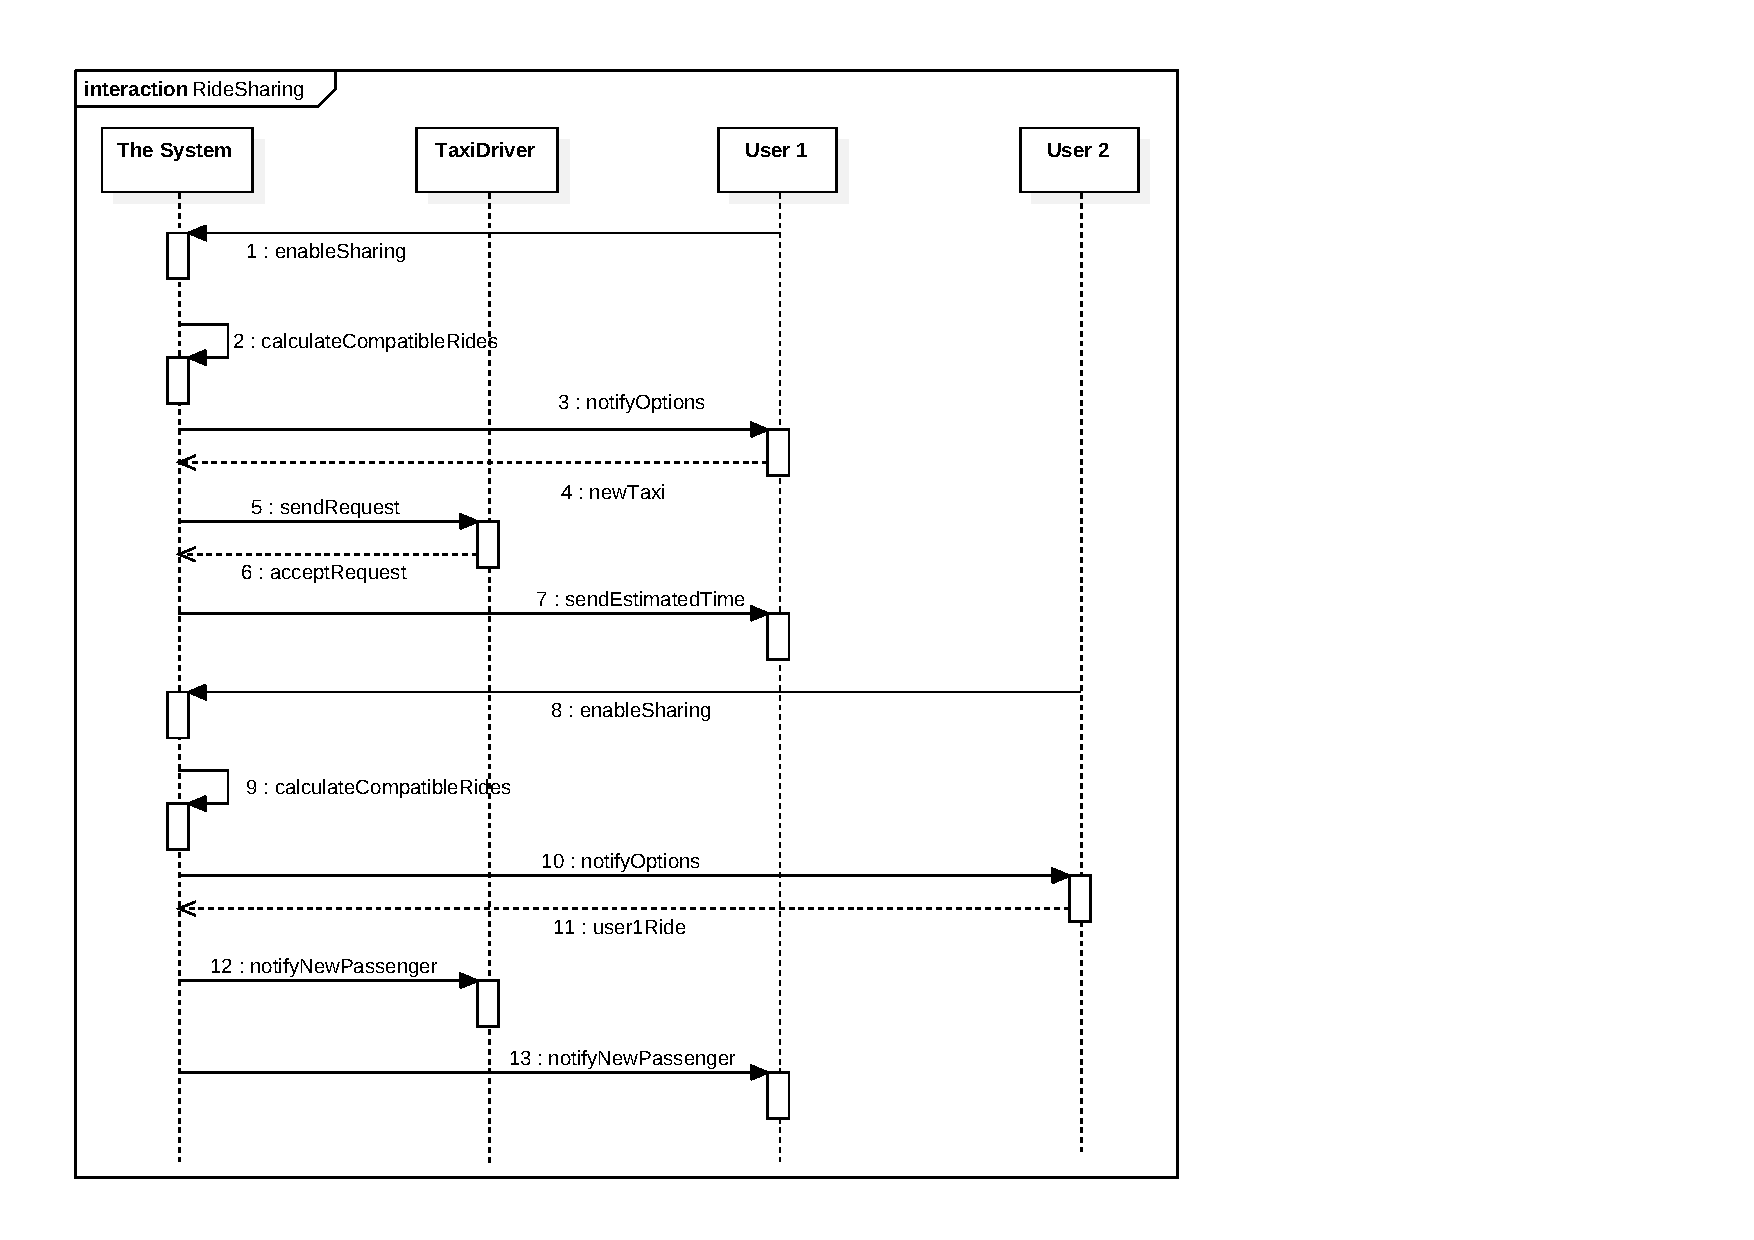
\includegraphics[width=\textwidth]{diagrams/sequence_ride_sharing.pdf}
	\caption{Sequence diagram of a ride sharing.}
	\label{fig:sequence-sharing}
\end{figure}

\subsubsection{Associated functional requirements}
\begin{enumerate}
\item The system has to know the starting point of the new passenger in order to provide feasible sharing solutions.
It has to compute the estimated walking time to reach the meeting location and compare it with the estimated taxi arrival time.
\item The passenger can enable the sharing function both in the mobile app and in the web interface.
\item The passenger can choose between possible sharing solutions or a new taxi.
\item The system has to communicate to the taxi driver the presence of a new passenger.
\item The system must be able to analyse the current sharing situation. % TODO too generic
\item The number of passenger must not exceed the number of seats available in each taxi.
\item The taxi driver can insert the number of passengers who have been picked up.
\item After the user chooses to enable the sharing mode, the system has to specify, for every sharing ride, the location and the time.
\end{enumerate}


\subsection{User profile management}
\label{user-profile}
\subsubsection{Purpose}
Any subscribed user can view or update his profile information.

The system allows taxi drivers to use the service only if they load a valid license. A reminder e-mail is sent to the taxi driver three months before the expiration.


\subsubsection{Scenario 1}
Alice, a myTaxiService passenger without a car, wants to count how many times she has used a taxi in the last month.
She opens the home page of myTaxiService page on the web site and clicks on ``login''.
After she has logged in correctly, she clicks on ``load profile'' and all the information about her account appears on screen, including the taxi request list.

\subsubsection{Scenario 2}
Gabriele's girlfriend has discovered his password but he doesn't want her to know where he has been. So he decides to change his password immediately. He opens the app on her cell phone, he selects ``load profile'' and after he selects ``modify password''. The system asks him to enter the old password and the new one two times to avoid errors. Once he has verified that everything's ok, he selects ``done'', and the system confirms that the password has been successfully set.

\subsubsection{Scenario 3}
A recall mail is sent to Bob, a myTaxiService user that has registered as taxi-driver, to notice him that he has to update his profile with a valid license. A week later he opens the app on his cell phone, he selects ``load profile'', then ``modify''. He enters the new license, then confirms selecting ``done''. The system confirms that the license has been successfully inserted.



\subsubsection{Use case}

The use case of profile management is illustrated in~\autoref{fig:usecase-profile}.
\begin{figure}
\begin{center}
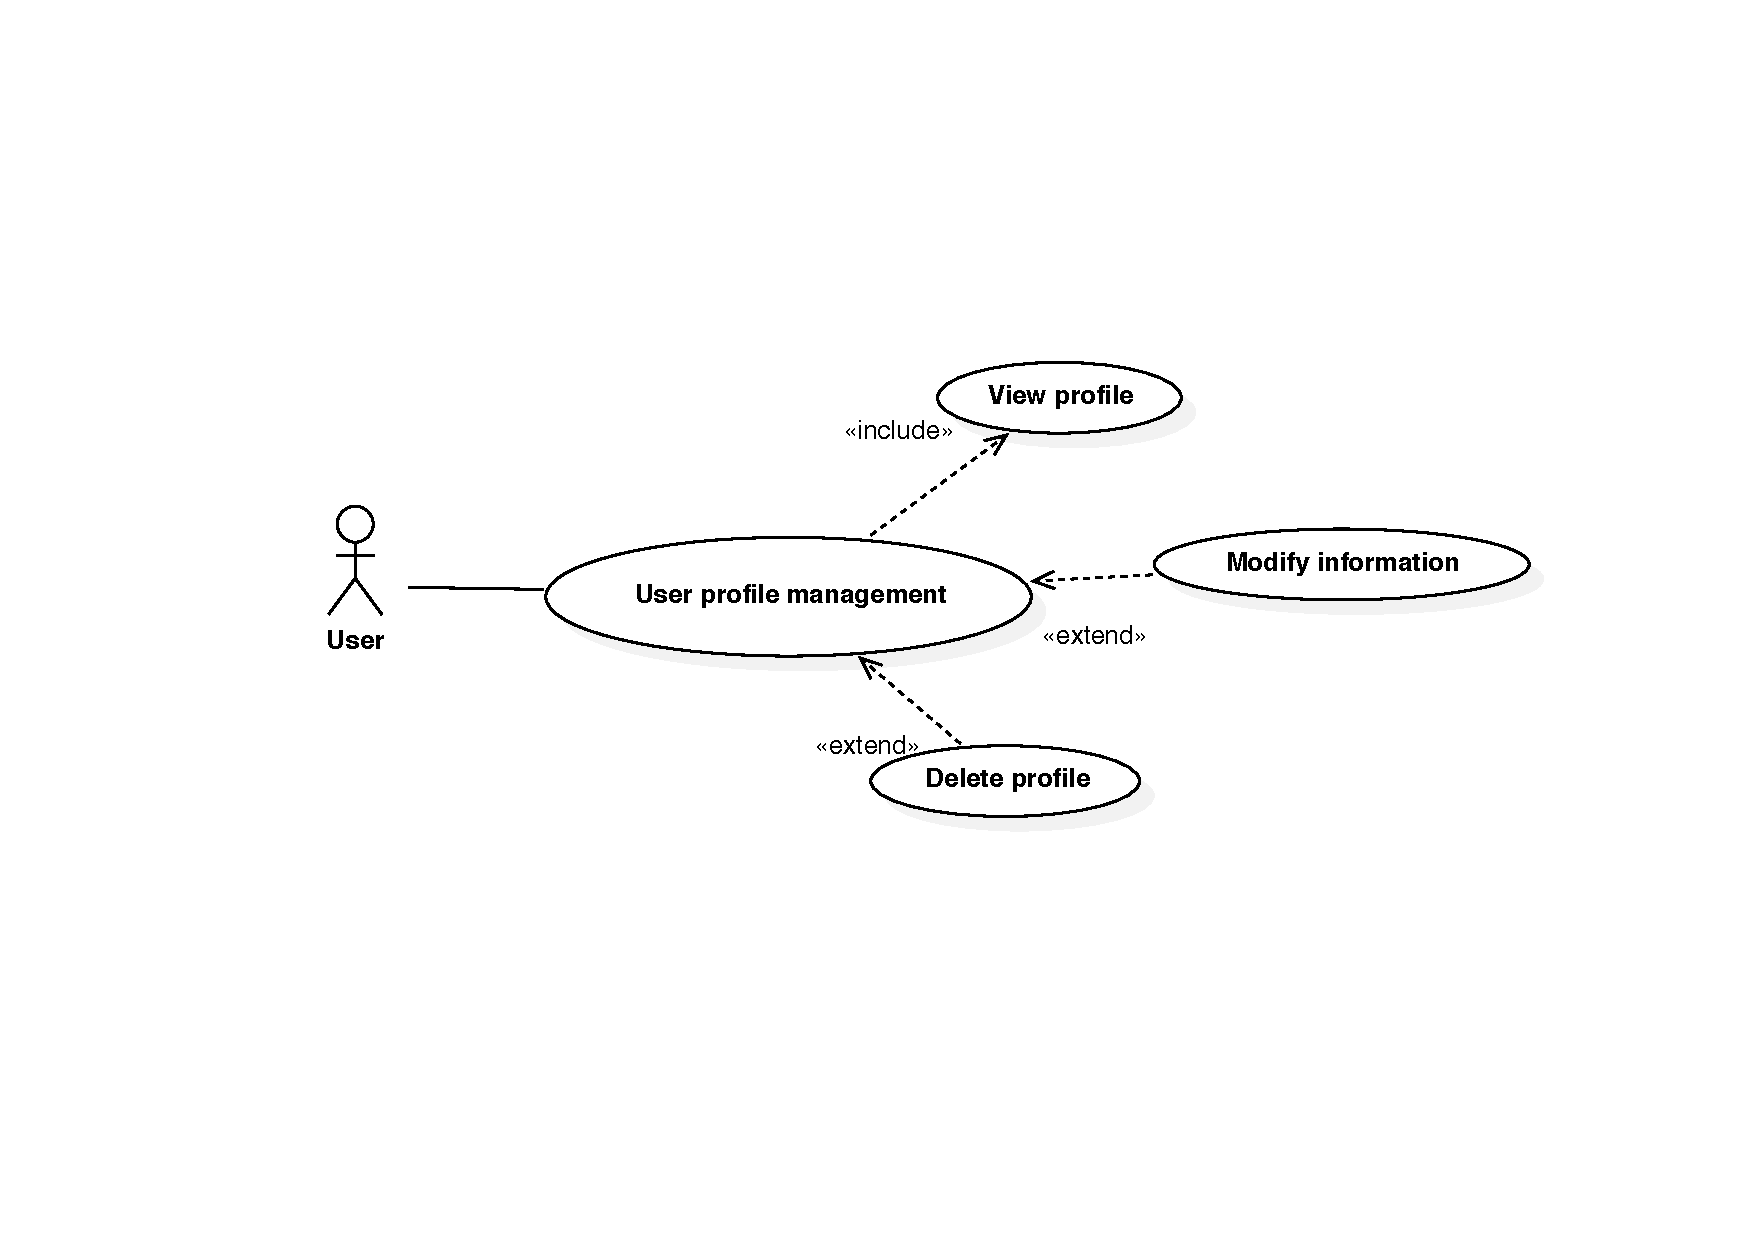
\includegraphics[width=0.7\textwidth]{diagrams/usecase_profile.pdf}
\caption{Use case diagram of user profile management.}
\label{fig:usecase-profile}
\end{center}
\end{figure}

The use case for viewing user profile is shown in~\autoref{usecase-profile-view}.

\begin{table}
\begin{center}
\begin{tabular}{| l | p{0.6\textwidth} |}
\hline
Actor & Registered user \\
\hline
Goal & Goal ~\ref{g-profile}
\\
\hline
Input condition & Passenger is already logged in and wants to check his profile.  \\
\hline
Event Flow & \begin{enumerate}
	\item The user selects load profile.
	\item The user's profile page is loaded.
	\end{enumerate}
\\
\hline
Output condition & The profile page is shown and the user can check his information. \\
\hline

Exception & None. \\
\hline
\end{tabular}
\end{center}
\caption{Use case for user profile visualization.}
\label{usecase-profile-view}
\end{table}



The use case for modifying the user profile is shown in~\autoref{usecase-profile-modify}.

\begin{table}
\begin{center}
\begin{tabular}{| l | p{0.6\textwidth} |}
\hline
Actor & Registered user \\
\hline
Goal & Goal ~\ref{g-profile}
\\
\hline
Input condition & Passenger is already logged in and wants to modify his profile.  \\
\hline
Event Flow & \begin{enumerate}
	\item The user selects load profile.
	\item The user's profile page is loaded.
	\item The user selects edit profile.
	\item The edit profile page is loaded.
	\item The user enters the new info.
	\item The user confirms
	\end{enumerate}
\\
\hline
Output condition & The information in the profile are updated. \\
\hline

Exception & If one of these requirements is not respected an exception occur:
\ref{f-modify-usrn1},
\ref{f-modify-usrn2},
\ref{f-modify-mail1},
\ref{f-modify-mail2},
\ref{f-modify-pswd1},
\ref{f-modify-pswd2},
\ref{f-modify-pswd3}.

The exception is handled ignoring the modified info, noticing the user and reloading the edit profile page. \\
\hline
\end{tabular}
\end{center}
\caption{Use case for user profile modification.}
\label{usecase-profile-modify}
\end{table}


The use case for deleting the user profile is shown in~\autoref{usecase-profile-delete}.

\begin{table}
\begin{center}
\begin{tabular}{| l | p{0.6\textwidth} |}
\hline
Actor & Registered user \\
\hline
Goal & Goal ~\ref{g-profile}
\\
\hline
Input condition & Passenger is already logged in and wants to delete his profile.  \\
\hline
Event Flow & \begin{enumerate}
	\item The user selects load profile.
	\item The user selects edit profile.
	\item The user selects delete profile.
	\item The systems asks the password.
	\item The user enters the password and confirms.
	\end{enumerate}
\\
\hline
Output condition & The user account is removed from the system database. \\
\hline

Exception & If the password entered is wrong, the user gets redirected to the ``edit profile'' page. \\
\hline
\end{tabular}
\end{center}
\caption{Use case for user profile deletion.}
\label{usecase-profile-delete}
\end{table}

\subsubsection{Associated functional requirements}
\begin{enumerate}

\item Logged passengers can:
\begin{itemize}
\item view user profile
\item modify an information
\item delete account
\item view the latest taxi request
\item view taxi requests list
\end{itemize}

\item Logged taxi drivers can:
\begin{itemize}
\item view user profile
\item modify an information
\item delete account
\item view the latest taxi request accepted
\item view requests accepted list
\end{itemize}

\item The system sends a recall mail three months before the expiration of the license submitted.

\item Delete the account:
\begin{enumerate}
\item The system allows to delete the user's account with an option on screen.
\item After ``delete account'' is selected, the user has to ensures his decision selecting on screen ``proceed'': the system deletes the account only after user's confirmation.
\item When an account is deleted all the relative information is destroyed.
\end{enumerate}

\item Modify the profile:
\begin{enumerate}
\item The system allows to change one or more information on the profile: any information can be changed, even the username or e-mail.
\item The system must verify that the new username entered is unique, i.e. there mustn't be another user that has already entered the same username.  \label{f-modify-usrn1}
\item  The system accept the new username only if it matches the regular expression\\``\texttt{[a-zA-Z][a-zA-Z0-9]\{2,20\}}''   \label{f-modify-usrn2}
\item The system must verify that the new e-mail entered is unique, i.e. there mustn't be another user that has already entered the same e-mail.   \label{f-modify-mail1}
\item If the e-mail is changed the system sends a confirmation mail on the new address.
\item The system saves the new mail only when the user clicks the link on the e-mail sent.   \label{f-modify-mail2}
\item The system accepts a new password that contains al least one number and one capital letter and that has a minimum length of eight characters.   \label{f-modify-pswd1}
\item The system accept a new password only if the old one has been submitted correctly before.  \label{f-modify-pswd2}
\item The system asks for the new password two times, when a user wants to change it.
\item The system accepts the new password only if the same one was entered twice.  \label{f-modify-pswd3}
\item The system must allow the user to abort the modification at any time.
\item The old information isn't  replaced until the ``done'' choice isn't selected by the user.
\end{enumerate}




\end{enumerate}


\section{Performance requirements}
The system must support at least 1000 connected passengers at once, and at least 500 simultaneously active taxi drivers at any given time.
95\% of requests shall be processed in less than 5 s; 100\% of requests shall be processed in less than 10 s.

There is no limit on the total number of registered users.

\section{Design constraints}
\subsection{Regulatory policies}
It's user responsibility to ensure that the use of the system complies with the local laws and policies.

The system must ask the user for the permission to acquire, store and process personal data and web cookies. The system must offer to the user the possibility to delete all the personal data.

\subsection{Hardware limitations}
the system has to run under the following conditions:
\begin{itemize}
\item App
\begin{itemize}
\item 3G connection, at 2 Mb/s
\item 100 MB of free space
\item 2 GB of RAM
\end{itemize}
\item Web application
\begin{itemize}
\item 2 Mb/s Internet connections
\item 800x600 resolution
\end{itemize}
\end{itemize}

\subsection{Reliability requirements}
The system must have a minimum availability of 98\%.

\subsection{Criticality of the application}
The system is not employed in life-critical applications.

\subsection{Safety and security considerations}
The locations of the passenger and its destinations must be kept private unless the passenger chooses to share rides.

Only taxi drivers with a valid license must be able to use the service for security reasons.


\section{Software system attributes}
% TODO Eleonora

\subsection{Reliability}
%This should specify the factors required to establish the required reliability of the software system at time of delivery.
\subsection{Availability}
%This should specify the factors required to guarantee a defined availability level for the entire system such as checkpoint, recovery, and restart.
\subsection{Security}
%This should specify the factors that protect the software from accidental or malicious access, use, modifica- tion, destruction, or disclosure. Specific requirements in this area could include the need to
%a) Utilize certain cryptographical techniques;
%b) Keep specific log or history data sets;
%c) Assign certain functions to different modules;
%d) Restrict communications between some areas of the program;
%e) Check data integrity for critical variables.
\subsection{Maintainability}
%This should specify attributes of software that relate to the ease of maintenance of the software itself. There may be some requirement for certain modularity, interfaces, complexity, etc. Requirements should not be placed here just because they are thought to be good design practices.
\subsection{Portability}
%This should specify attributes of software that relate to the ease of porting the software to other host machines and/or operating systems. This may include the following:
%a) Percentage of components with host-dependent code;
%b) Percentage of code that is host dependent;
%c) Use of a proven portable language;
%d) Use of a particular compiler or language subset;
%e) Use of a particular operating system.

\section{Other requirements}
\input{specific_requirements/other_requirements.tex}

\end{document}
